\documentclass{article}


\usepackage{arxiv}

\usepackage[utf8]{inputenc} % allow utf-8 input
\usepackage[T1]{fontenc}    % use 8-bit T1 fonts
\usepackage{hyperref}       % hyperlinks
\usepackage{url}            % simple URL typesetting
\usepackage{booktabs}       % professional-quality tables
\usepackage{amsfonts}       % blackboard math symbols
\usepackage{nicefrac}       % compact symbols for 1/2, etc.
\usepackage{microtype}      % microtypography
\usepackage{lipsum}
\usepackage{amsmath}

\usepackage{graphicx}
\usepackage{graphics}
\usepackage{float}
\usepackage{subfigure}
\usepackage{multirow}

\title{Urban Vibrancy and Land Zoning Influences on the Crime Effects of Vacant Lot Greening}


\author{
  Jesse Cui \\
  Wharton Social Impact Initiative\\
  The Wharton School, University of Pennsylvania\\
  Philadelphia, PA 19104 \\
  \texttt{jessecui@wharton.upenn.edu} \\
  %% \AND
  %% Coauthor \\
  %% Affiliation \\
  %% Address \\
  %% \texttt{email} \\
  %% \And
  %% Coauthor \\
  %% Affiliation \\
  %% Address \\
  %% \texttt{email} \\
  %% \And
  %% Coauthor \\
  %% Affiliation \\
  %% Address \\
  %% \texttt{email} \\
}

\begin{document}
\maketitle

\begin{abstract}
The city of Philadelphia has been recently interested in observing the crime and safety effects of greening intervention on vacant lots within neighborhoods. Using available Philadelphia vacant lot and crime datasets, we assign violent and non-violent crime counts to lots over a decade-long time-span. We then characterize lots with publicly available demographic, economic, land use, and business vibrancy data. We use propensity scoring on whether a lot is greened to control for covariates and perform a matched pairs t-test to analyze the influence of greening on crime. We then cluster our dataset by land use zoning percentages to observe which areas are more or less likely to be influenced by greening intervention in terms of crime. Similarly, we then cluster our dataset by business vibrancy characteristics to observe which areas are more or less likely to be influenced by certain businesses in the neighborhood. Overall we find that greening intervention on a vacant lot, when compared to another vacant lot with equal propensity to be treated but without greening intervention, shows significant decreases in crimes for both violent and non-violent crimes using a difference-in-differences design. More specifically, we find that greening lots in areas with high residential, high civic/institutional, low commercial, and low transportation areas have a higher effect in decreasing crimes. We also find that greening lots in areas with pharmacies and convenience stores have a higher effect in decreasing crimes.
\end{abstract}


% keywords can be removed
\keywords{urban analytics \and business vibrancy \and vacant lot greening \and crime}


\section{Introduction}
Cities such as Philadelphia are facing a large number of unused, vacant lots. A large amount of prior works have analyzed the effects of converting vacant lots into greened spaces on the surrounding neighborhood of the lot. In particular, prior research has analyzed the effects of vacant lot greening on violent and non-violent neighborhood crimes. The efforts started with Branas et al. performing a decade-long difference-in-differences analysis of the impact of vacant lot greening in Philadelphia and found consistent reductions in gun assaults in all sections of the city and reductions in vandalism in one section of the city \cite{branas-1}.  This work was continued through Garvin et al., which found a decrease, although non-significant, in the number of total crimes and gun assaults around greened vacant lots compared with control using unadjusted difference-in-difference estimates \cite{garvin-1}. Kondo et al. used regression models adjusted for spatial autocorrelation and found the most consistent significant reductions in burglaries and in assaults around greened lots \cite{kondo-1}.

Effects beyond crime have been explored as well. Economic benefits have been shown. Heckert and Mennis used spatial difference-in-differences analysis and saw that property values surrounding greened vacant lots had a greater increase in value than properties surrounding non-greened vacant lots \cite{heckert_mennis-1}. Furthermore, these researchers have also established a link between greened lots and the health and well-being of the residents in an area. Branas et al. also found that within certain parts of the city, vacant lot greening was associated with residents reporting less stress and more exercise \cite{branas-1}. Garvin et al. saw that people around intervention vacant lots report feeling significantly safer after greening compared to those living around controlled vacant lots \cite{garvin-1}. South et al. discovered that being in view of a greened vacant lot decreased heart rate significantly more than being in the view of a non-greened vacant lot, and concluded that remediating neighborhood blight may reduce stress and improve health \cite{south-1}. Feelings of depression and self-reported poor mental health were reduced in participants living near greened vacant lots \cite{south-2}. 

The purpose of this paper is to perform propensity scoring and matching on land-use zoning and business vibrancy characteristics of neighborhoods and then analyze the effects of greening intervention on matched pairs of vacant and treated lots. We will continue the controlled analysis of crime differences in greened versus non-greened vacant lots; however, we will also use new data features such as land use zoning data and business vibrancy data to control and cluster our data.

\section{Processing Urban Data in Philadelphia}
\subsection{Datasets Used}

A total of 9 datasets were used.

\begin{enumerate}
\item \textbf{Crime Dataset} \\
We retrieved Philadelphia crime data in the years 2007 to 2019 via OpenDataPhilly. This dataset gets updated frequently from the Philadelphia police department. We filtered the crimes to exclude types of crimes that are not relevant or intuitive to greening interventions, such as embezzlement, narcotics, and gambling. We ended up with 1496015 crimes after filtering. Crimes were then further categorized into two types. The first type is \textbf{violent crimes}, which contain homicides, rapes, robberies, and aggravated assaults. The second type of crimes is \textbf{non-violent crimes}, which contains burglary, thefts, vehicle thefts, other assaults, arson, vandalism, offenses against family and children, public drunkenness, disorderly conduct, and vagrancy/loitering.
\item \textbf{Greened Lots Dataset}\\
Greened vacant lot data used in this study was taken from the Pennsylvania Horticultural Society's Land Care program and were subsetted between the data range of 9/01/2007 - 9/01/2017. Greened lots were filtered to exclude entries that contained null or non-existent data. We ended up with 4651 lots after filtering.
\item \textbf{Vacant Lots Dataset}\\
Non-greened vacant lot data used in this study is filtered from the Philadelphia's Licenses and Inspections Office. Lots were filtered to exclude entries that contained null or non-existent data, and were also filtered through the date ranges of  9/01/2007 - 9/01/2017. The retrieved list of violations is filtered to only include violations that are vacant property (non-building) violations. We also filtered out duplicate violations locations to only include the first violation instance of each vacant land violation case. We ended up with 16799 vacant lots after filtering.
\textbf{\item Census Block Demographic Dataset}\\
Demographic data for Philadelphia is taken from the U.S. Census, which includes data on census block population size and racial proportions. The exact dataset is 2010 Decennial Census SF1 100\% Data, All Blocks within Philadelphia County, Pennsylvania Table P5: HISPANIC OR LATINO ORIGIN BY RACE.
\textbf{\item  Per Capita Income Economic Dataset}\\
Economic data for Philadelphia is taken from the American Community Survey, which includes per capita income for census blocks in Philadelphia. The exact dataset is 2015 ACS 5-year estimates for Philadelphia County (Blockgroup resolution). Table B19301: PER CAPITA INCOME IN THE PAST 12 MONTHS (IN 2015 INFLATION-ADJUSTED DOLLARS).
\textbf{\item  Census Block Ratio of Income to Poverty Level Economic Dataset}\\
Economic data for Philadelphia is taken from the American Community Survey, which includes income to poverty ratios for census blocks in Philadelphia. The exact dataset is 2015 ACS 5-year estimates for Philadelphia County (Blockgroup resolution). Table C17002: RATIO OF INCOME TO POVERTY LEVEL IN THE PAST 12 MONTHS.
\textbf{\item Land Zoning Dataset}\\
We also retrieved Land Zoning Data from OpenDataPhilly. We aggregated the zones into eight main groups, listed in table \ref{tab:land_use_cat}.
\begin{table}[h]
  \begin{center}
    \caption{Land Use Categories}
    \label{tab:land_use_cat}
    \begin{tabular}{c}
      \toprule % <-- Toprule here
      Residential\\
      Commercial\\
      Industrial\\
      Civic/Inst\\
      Transportation\\
      Cultural/Park\\
      Water\\
      Vacant\\
      Other\\
      \bottomrule % <-- Bottomrule here
    \end{tabular}
  \end{center}
\end{table}
\textbf{\item Census Block Group Dataset}\\
We also retrieved Census Block Group data from OpenDataPhilly. This data is used to join the lots datasets to the economic, demographic, and land zoning data on a block level.
\textbf{\item Business Vibrancy Dataset}\\
We retrieved business vibrancy data for Philadelphia from prior research done by the Wharton Statistics Department \cite{humphrey2017urban}. This dataset contains information of the locations of businesses under the categories listed in table \ref{tab:bus_vib_cat}.
\begin{table}[h]
  \begin{center}
    \caption{Business Vibrancy Categories}
    \label{tab:bus_vib_cat}
    \begin{tabular}{c}
      \toprule % <-- Toprule here
      Cafe\\
      Convenience\\
      Gym\\
      Institution\\
      Liquor\\
      Lodging\\
      Nightlife\\
      Pharmacy\\
      Restaurant\\
      Retail\\
      \bottomrule % <-- Bottomrule here
    \end{tabular}
  \end{center}
\end{table}
\end{enumerate}
% TODO Add Math Equations as well as beef up certain sections
\subsection{Data Preprocessing Methods}
The goal of the project is to assign economic, demographic, land zoning, and business attributes to each greened lot and non-greened vacant lot. After preprocessing data in this manner, the lots will be fed into a propensity scoring model to assign each lot a score on its propensity to be greened, based on its locational features. Lots will then be paired based on their propensity scores, and a matched pairs t-test will be performed to analyze the significance of crime effect with greening intervention.\\\\
\textbf{Calculating Crimes Surrounding Each Lot}\\
Using Python scripts, crimes were attached to each lot based on whether they fill within a certain radius from the center of the lot. Three radii values were used: 100 meters, 200 meters, and 500 meters. Distances were calculated from GPS coordinates using Vincenty's formula. We counted crimes before the greening intervention as crimes that occurred 6 to 18 months before the lot was greened, and we counted crimes after the greening intervention as crimes that occurred 6 to 18 months after the lot was greened. Note that we excluded a one year period around the greening period of the lot, as the intervention data was accurate only to a 6 month period. \\\\
Furthermore, we noticed that our vacant lots overlapped some of our greened lots in terms of coordinates. This implies that our vacant lots dataset included greened lots before intervention occurred. To ensure that there is mutual exclusivity between treated and control lots, we further filtered our vacant lots dataset to ensure that there is no greened lot whose coordinate is within 50 meters of a vacant lot. \\\\
\textbf{Calculating Economic and Demographic Characteristics Per Lot}\\
Using Python scripts, economic and demographic features were appended to the lots on the census block level. For the demographic data, we used data out of the primary four racial groups: black, white, hispanic, and asian. Overall, for each lot, we have data on the racial proportions, population, per capita income, and income to poverty ratios of the census block surrounding the lot.\\\\
\textbf{Calculating Land Use Zoning Surrounding Each Lot}\\
Using Python scripts and packages for shapefiles, lots were assigned land use zoning characteristics. Specificly, a circle with a specified radius was drawn around each lot's coordinates, and the percentage of each land use type of in this circular area was recorded for each lot. The steps to create this dataset are described as follows:
\begin{enumerate}
    \item Group all land use zones into the eight aforementioned categories
    \item Union all land use zones in each land use category $i$. Let $z_i$ denote a zone $z$ with land use category characteristic $i$.
        \begin{equation}
            \text{Unioned.Area}_i =  \bigcup{z_i}
        \end{equation}
    \item For each lot, calculate the area for each land use zone category as follows
        \begin{enumerate}
            \item For a given radius $r$ (we used 200 meters), given a land use zone category $i$, intersect the unioned zone shape with the $r$ radius circle around the lot. Let $r_l$ denote the $r$ radius circle surrounding a lot $l$.
            \item Calculate the area of this intersection
            \begin{equation}
                Area(\text{Land.Use.Category.}_i) =  \text{Unioned.Area}_i \bigcap Area(r_l)
            \end{equation}
            \item Divide this intersection area by the area of a $r$ radius circle to get the proportion of the lot $l$ that is the specific land use type $i$
            \begin{equation}
                \text{Land.Use.Category.Prop}_i = \frac{Area(\text{Land.Use.Category}_i)}{\pi * r^2}
            \end{equation}
        \end{enumerate}
\end{enumerate}
We calculated the proportion of a lot that is residential by subtracting the sum of the proportions of all other land use types by 1.\\\\
\textbf{Calculating Business Vibrancy Surrounding Each Lot}\\
We calculated business vibrancy characteristics per lot with indicator variables denoting whether each business type was present in a 200 meter radius from each lot’s coordinates. We also included the total number of businesses in the region. The steps to determine indicator variables for this dataset are described as follows:
\begin{enumerate}
    \item Group all business vibrancy categories into the ten aforementioned categories
    \item For each lot $l$, given radius $r$ (we used 200 meters), and given a business characteristic $i$, denote whether there exists one business $b$ with attribute $i$ in the $r$ radius circle surrounding lot $l$, which we will denote as $r_l$. Let $b_i$ denote a the coordinates of business $b$ with business characteristic $i$. 
    \begin{equation}
        \text{Contains.Attribute.}i =
        \begin{cases}
        1, & \exists b_i \in r_l \\
        0, & \text{otherwise}
        \end{cases}
    \end{equation}
\end{enumerate}
\section{Summary Data Analysis on Vacant and Treated Lots}
\subsection{Naive t-tests Between Mean Crime Differences of Treated and Control Lots}
    For greened lots, we processed crimes in a 6 to 18 month window, or 180 to 545 day window, before and after the intervention date. We also calculated the same window of crimes for our vacant lots. However, since vacant lots do not have an inherent greening lot date, we decided for exploratory comparisons to treated lots that we use the average greening intervention date as the control intervention date (we will discuss a better way to control for differences between treated and untreated lots soon). This average intervention date is October 30th, 2012. Displayed in Figure \ref{fig:figure1} are box and whisker plots comparing crimes at a 200m radius before and after a greening intervention.
    \begin{figure}[h]
    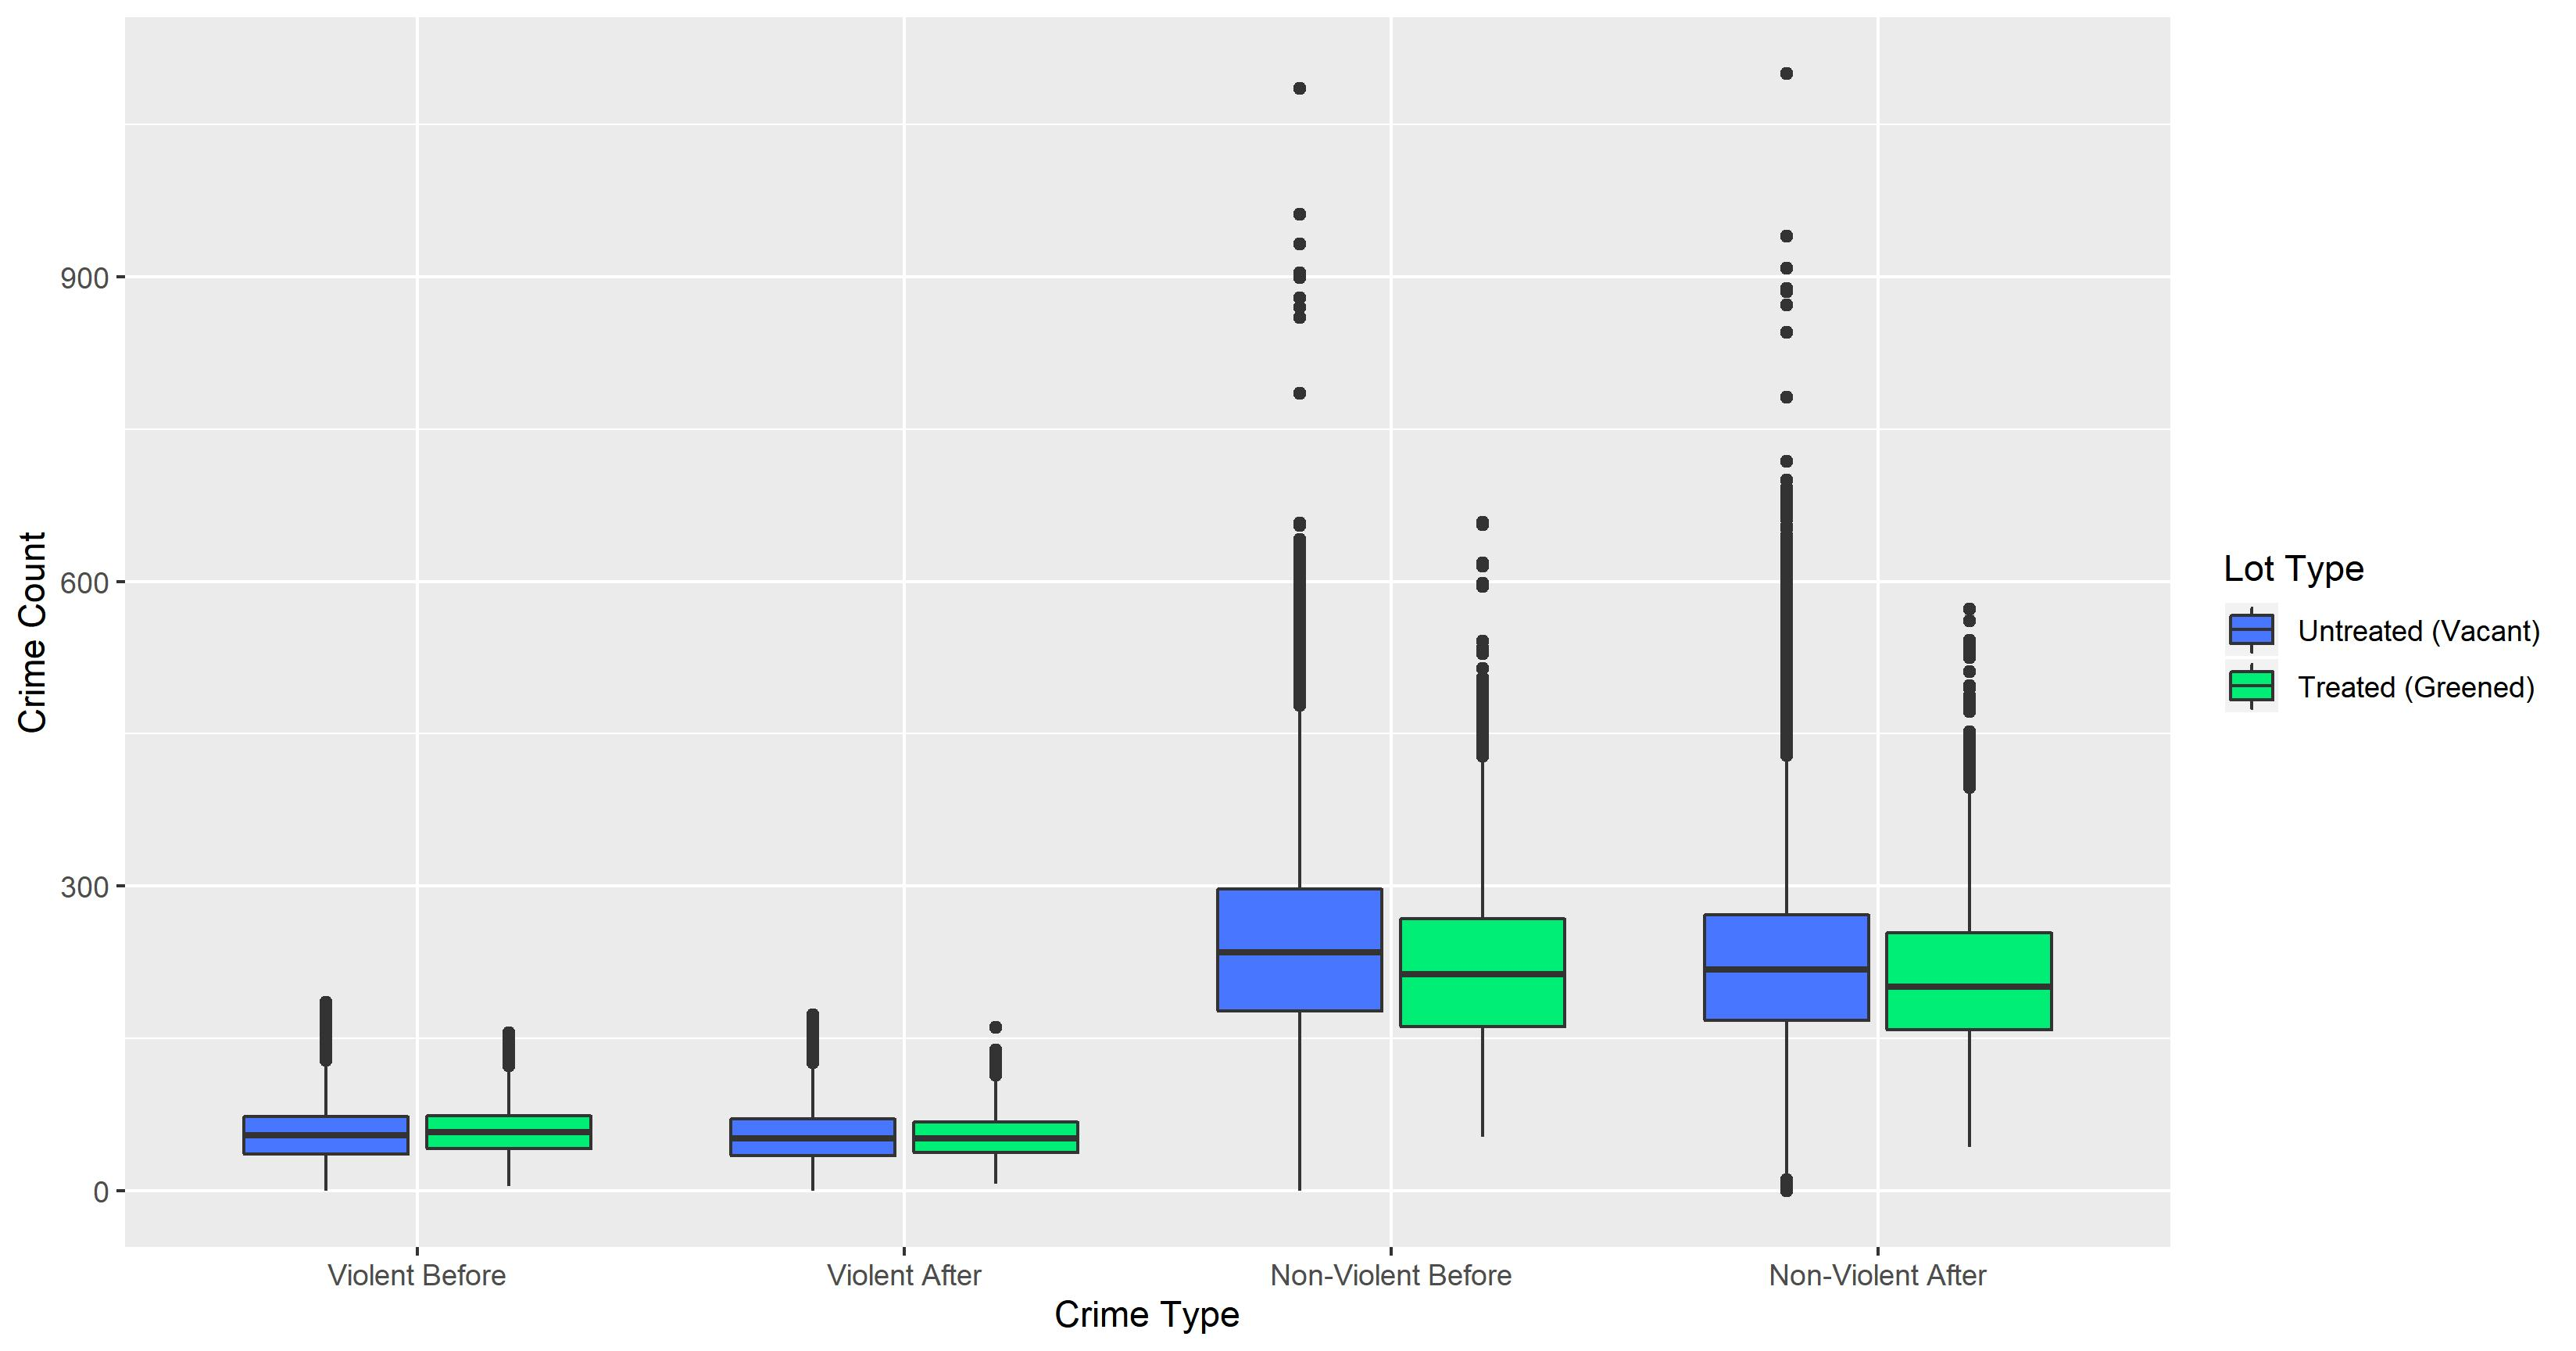
\includegraphics[width=12cm]{imgs/chart_crimes_before_match_200.jpg}
    \centering
    \caption{Violent and non-violent crime counts within 200m radius of greening intervention}
    \label{fig:figure1}
    \end{figure}
    
   We then performed a simple difference-in-differences statistical test using a t-test of means, comparing crimes drops between vacant and treated lots. The results are shown in table \ref{tab:nonpair-t-test}.
   \begin{table}[h]
   \begin{center}
   \caption{\label{tab:nonpair-t-test}Non-paired t-tests on Crime Difference-in-Differences Between Greened and Vacant lots}
    \begin{tabular}{lllllll}
    \hline
    \textbf{t}            & \textbf{p}  & \textbf{Greened Mean} & \textbf{Vacant Mean} & \textbf{DOD} & \textbf{Crime Type} & \textbf{Radius} \\ \hline
    \textbf{-0.362389113} & 0.717074046 & -4.87486562         & -4.758861957         & -0.116003663 & total         & 100             \\
    \textbf{5.419002388}  & 6.23E-08    & -16.19329177        & -20.1373291          & 3.944037332  & total         & 200             \\
    \textbf{10.21716146}  & 2.72E-24    & -103.9602236        & -127.8200835         & 23.85985992  & total         & 500             \\
    \end{tabular}
    \end{center}
    \end{table}
    With a naive, non-paired simple t-test of means between the crime difference before and after greening intervention with the control difference for non-greened vacant lots, we see a significant increase in crimes differences with greening intervention compared to the control when calculating crimes at a 200 meter and 500 meter radius surrounding the lot, using a significance level of 0.05. We do not see significance at the 100 meter radius level. At first, it seems that greening intervention does not help reduce crime compared to the control.
    
    Limited conclusions can be drawn from these results due to hidden biases and confounding variables. There are many biases that can influence these results. For example, the control date to measure the difference before and after greening intervention for vacant lots was set to be the average greening intervention date. Because all differences in crimes were measured with the same date for vacant lots, the discrepancy in the level of crimes surrounding that one date compared to other dates can heavily persuade the results.
    
    If we graph the level of crimes against the level of greening as shown in figure \ref{fig:figure2}, we see that there is variability between when lots are greened and when crimes occur. In fact, many greening interventions occurred in 2016, where there were low amounts of crimes. We also see that in the year 2012 that there was a large drop in crimes, yet not many lots were greened during this year. It's not a fair analysis to compare crime drops for vacant lots in a really good year for crime decreases to the crime drops for greened lots which occur throughout multiple years. 
    
    \begin{figure}[h]
    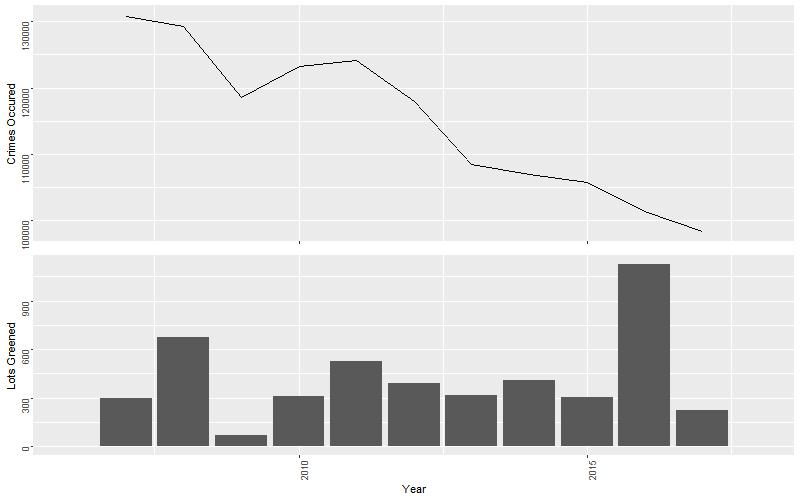
\includegraphics[width=10cm]{imgs/chart_crime_vs_green_lots.jpg}
    \centering
    \caption{Crimes Dispatched and Lots Greened By Year}
    \label{fig:figure2}
    \end{figure}
    
    Another source of hidden bias is the potential for lots chosen to be treated and greened to have specific and different neighborhood characteristics than those not selected to be greened. In this upcoming section, we will soon observe variability along different characteristics between lots chosen to be treated and lots not chosen to be treated.
    
\subsection{Characteristic Differences Between Greened and Vacant Lots}
\begin{enumerate}
    \item \textbf{Demographic Comparisons for Lots} \\\\
    Figure \ref{fig:figure3} shows a box and whisker plot comparing demographic characteristics between vacant lots without greening and greened lots. The data suggests that neighborhoods surrounding greened lots have a lower proportion of hispanics and whites than neighborhoods surrounding lots that have not been greened but have higher proportions of blacks.
    
    \begin{figure}[h]
    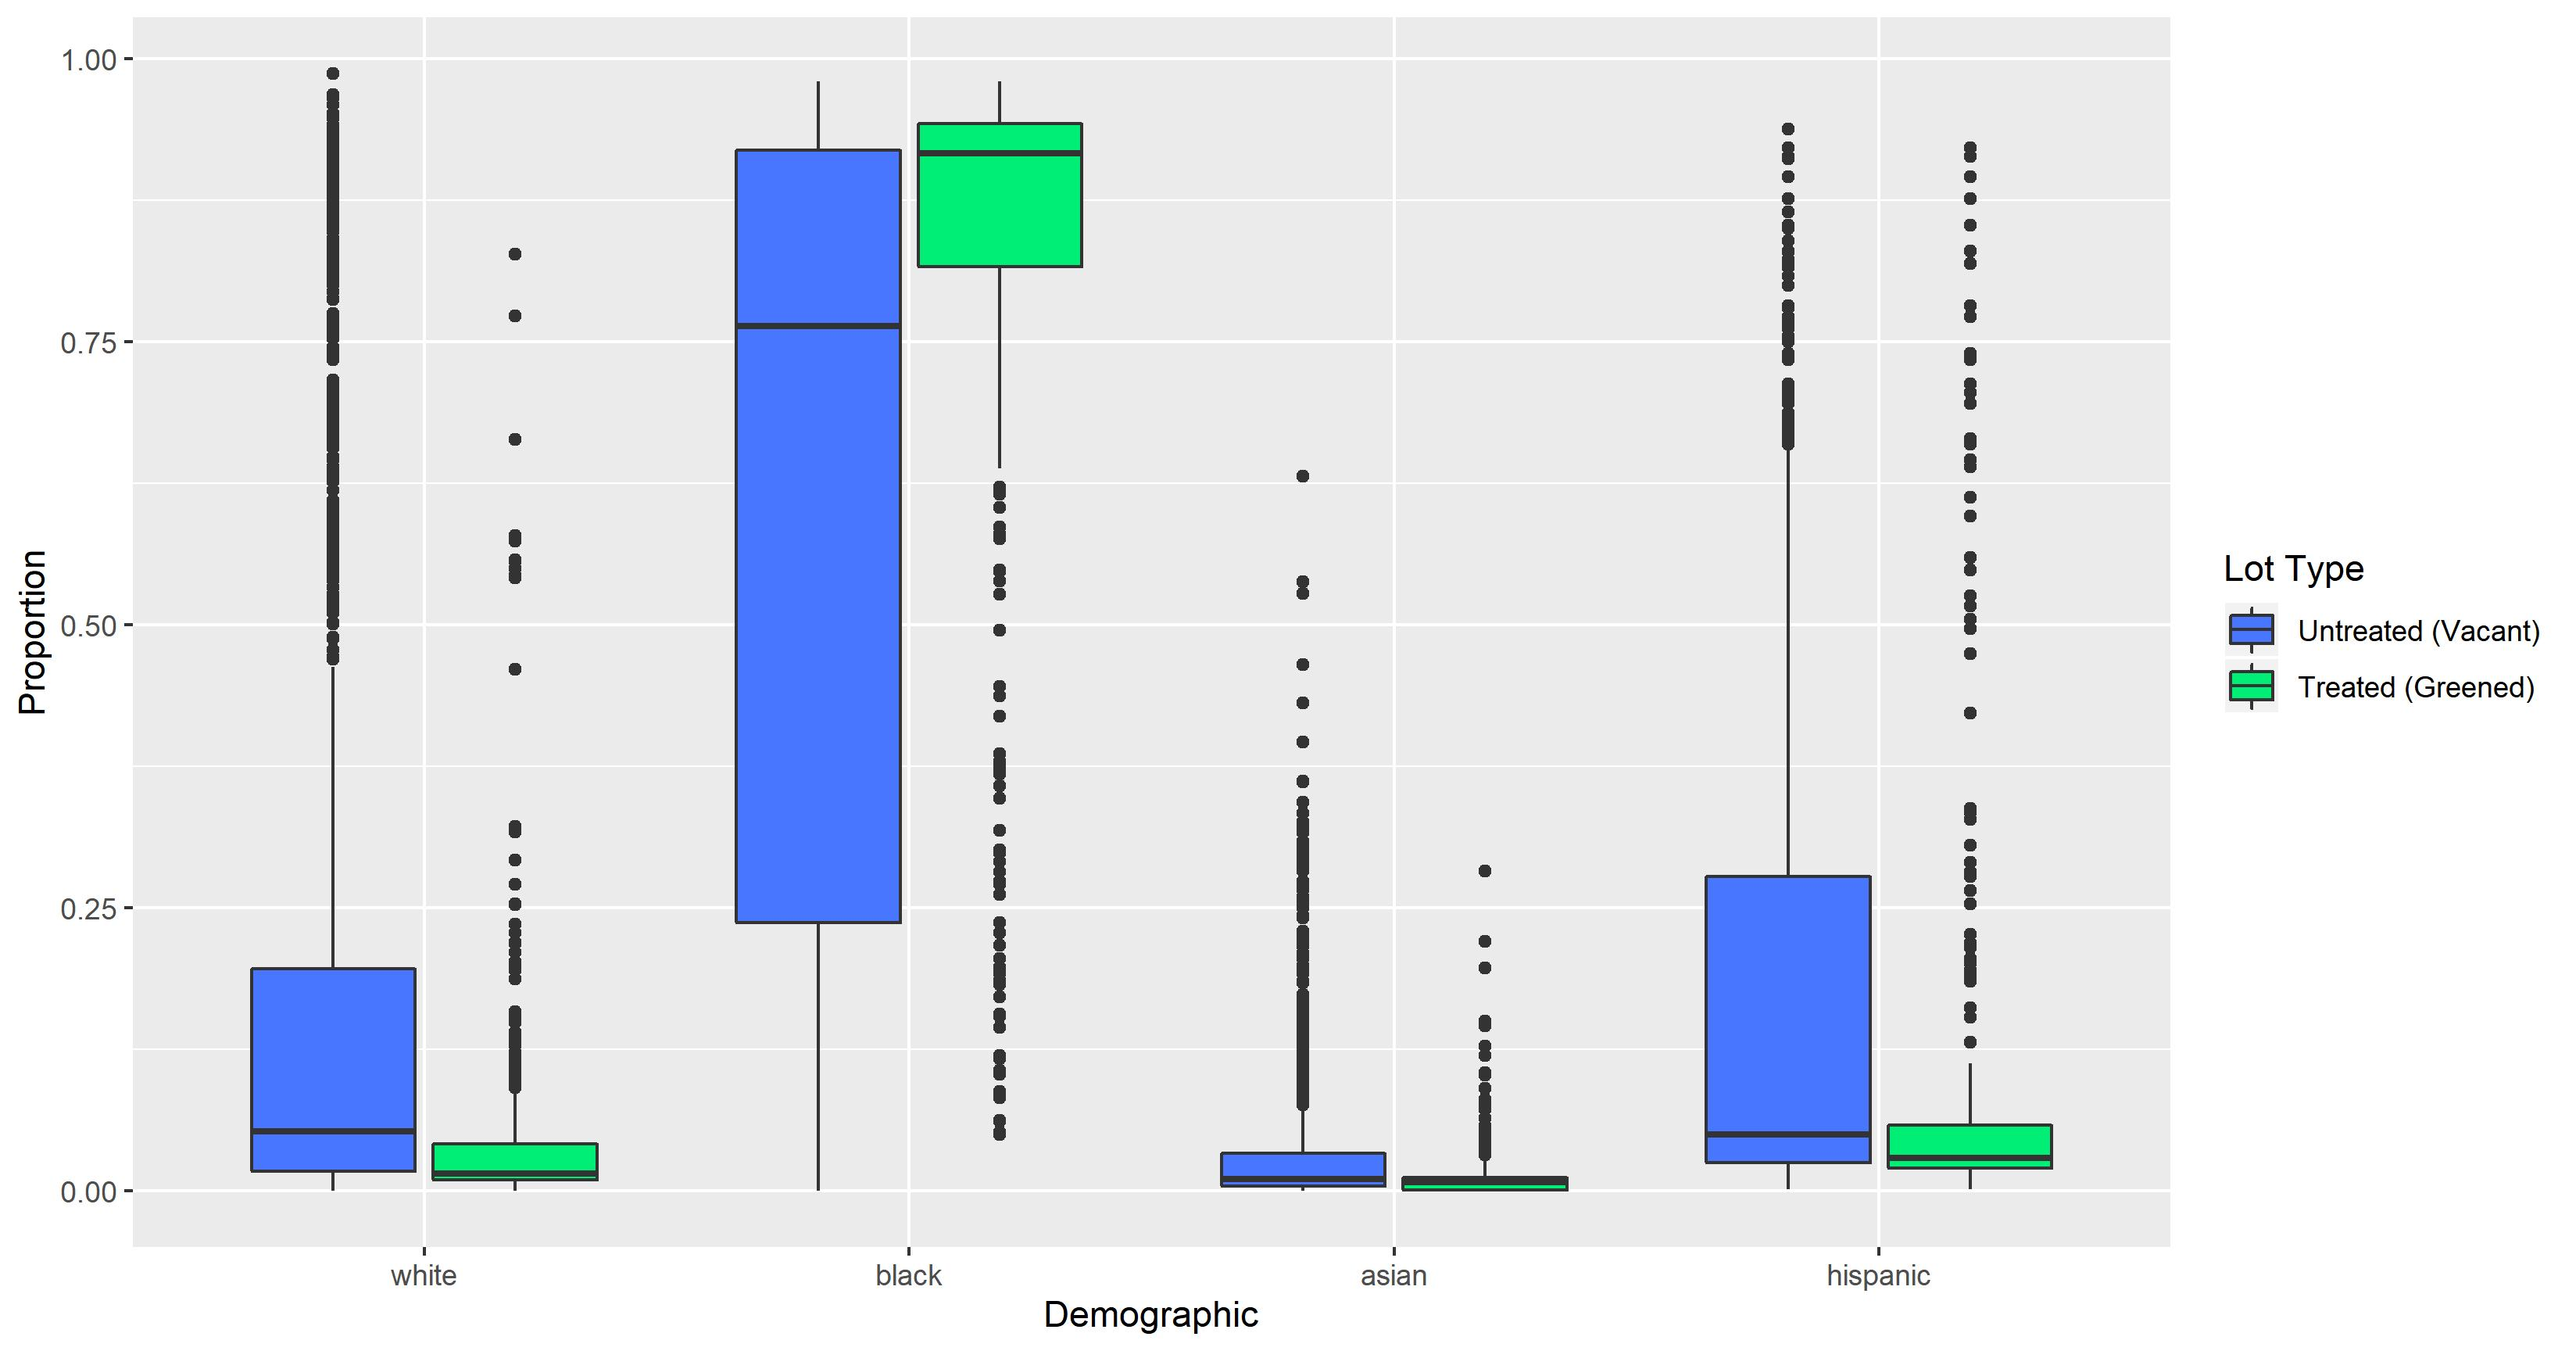
\includegraphics[width=10cm]{imgs/chart_demog.jpg}
    \centering
    \caption{Ethnic Proportions for Census Blocks Surrounding Lots}
    \label{fig:figure3}
    \end{figure}
    
    Figure \ref{fig:figure4} shows a box and whisker plot comparing the population size between vacant lots without greening and greened lots. The data suggests that greened lots tend to occur in smaller neighborhoods due to a larger skew towards smaller block populations.
    
    \begin{figure}[h]
    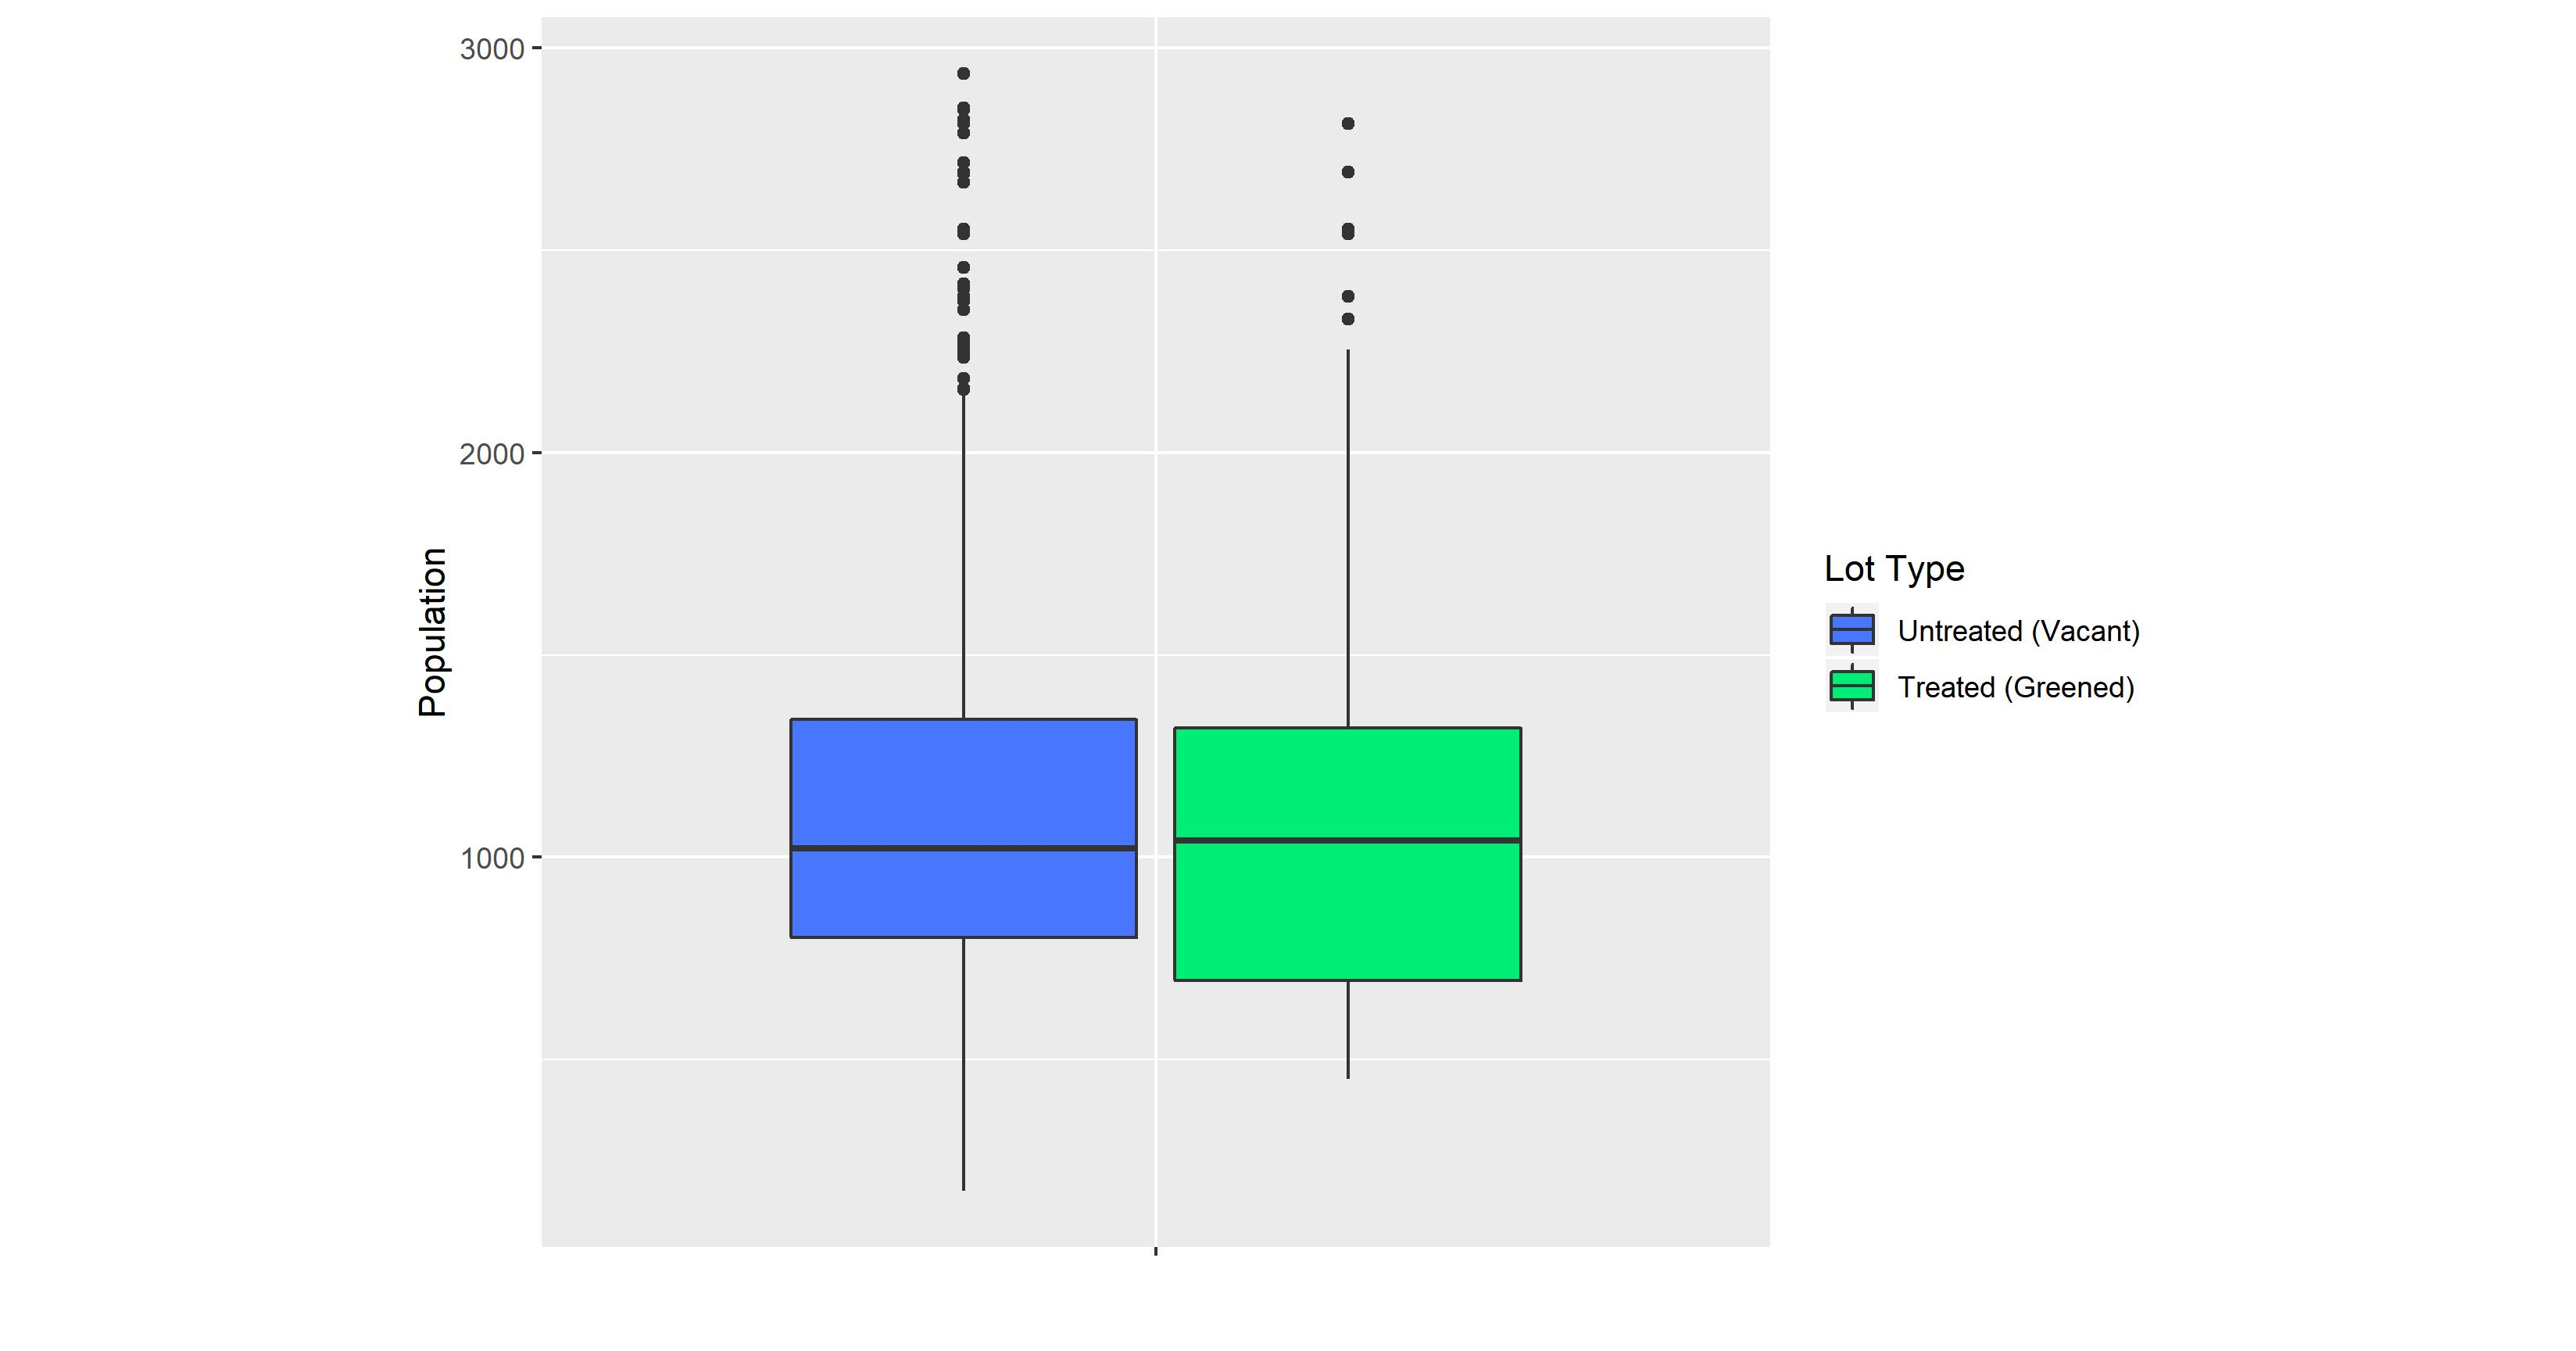
\includegraphics[width=10cm]{imgs/chart_pop_count.jpg}
    \centering
    \caption{Population Count Distribution for Lots}
    \label{fig:figure4}    
    \end{figure}

    \item \textbf{Economic Comparisons for Lots} \\
    Figure \ref{fig:figure5} displays a box and whisker plot comparing the per capita income between vacant lots without greening and greened lots as well as statistics.
    \begin{figure}[h]
    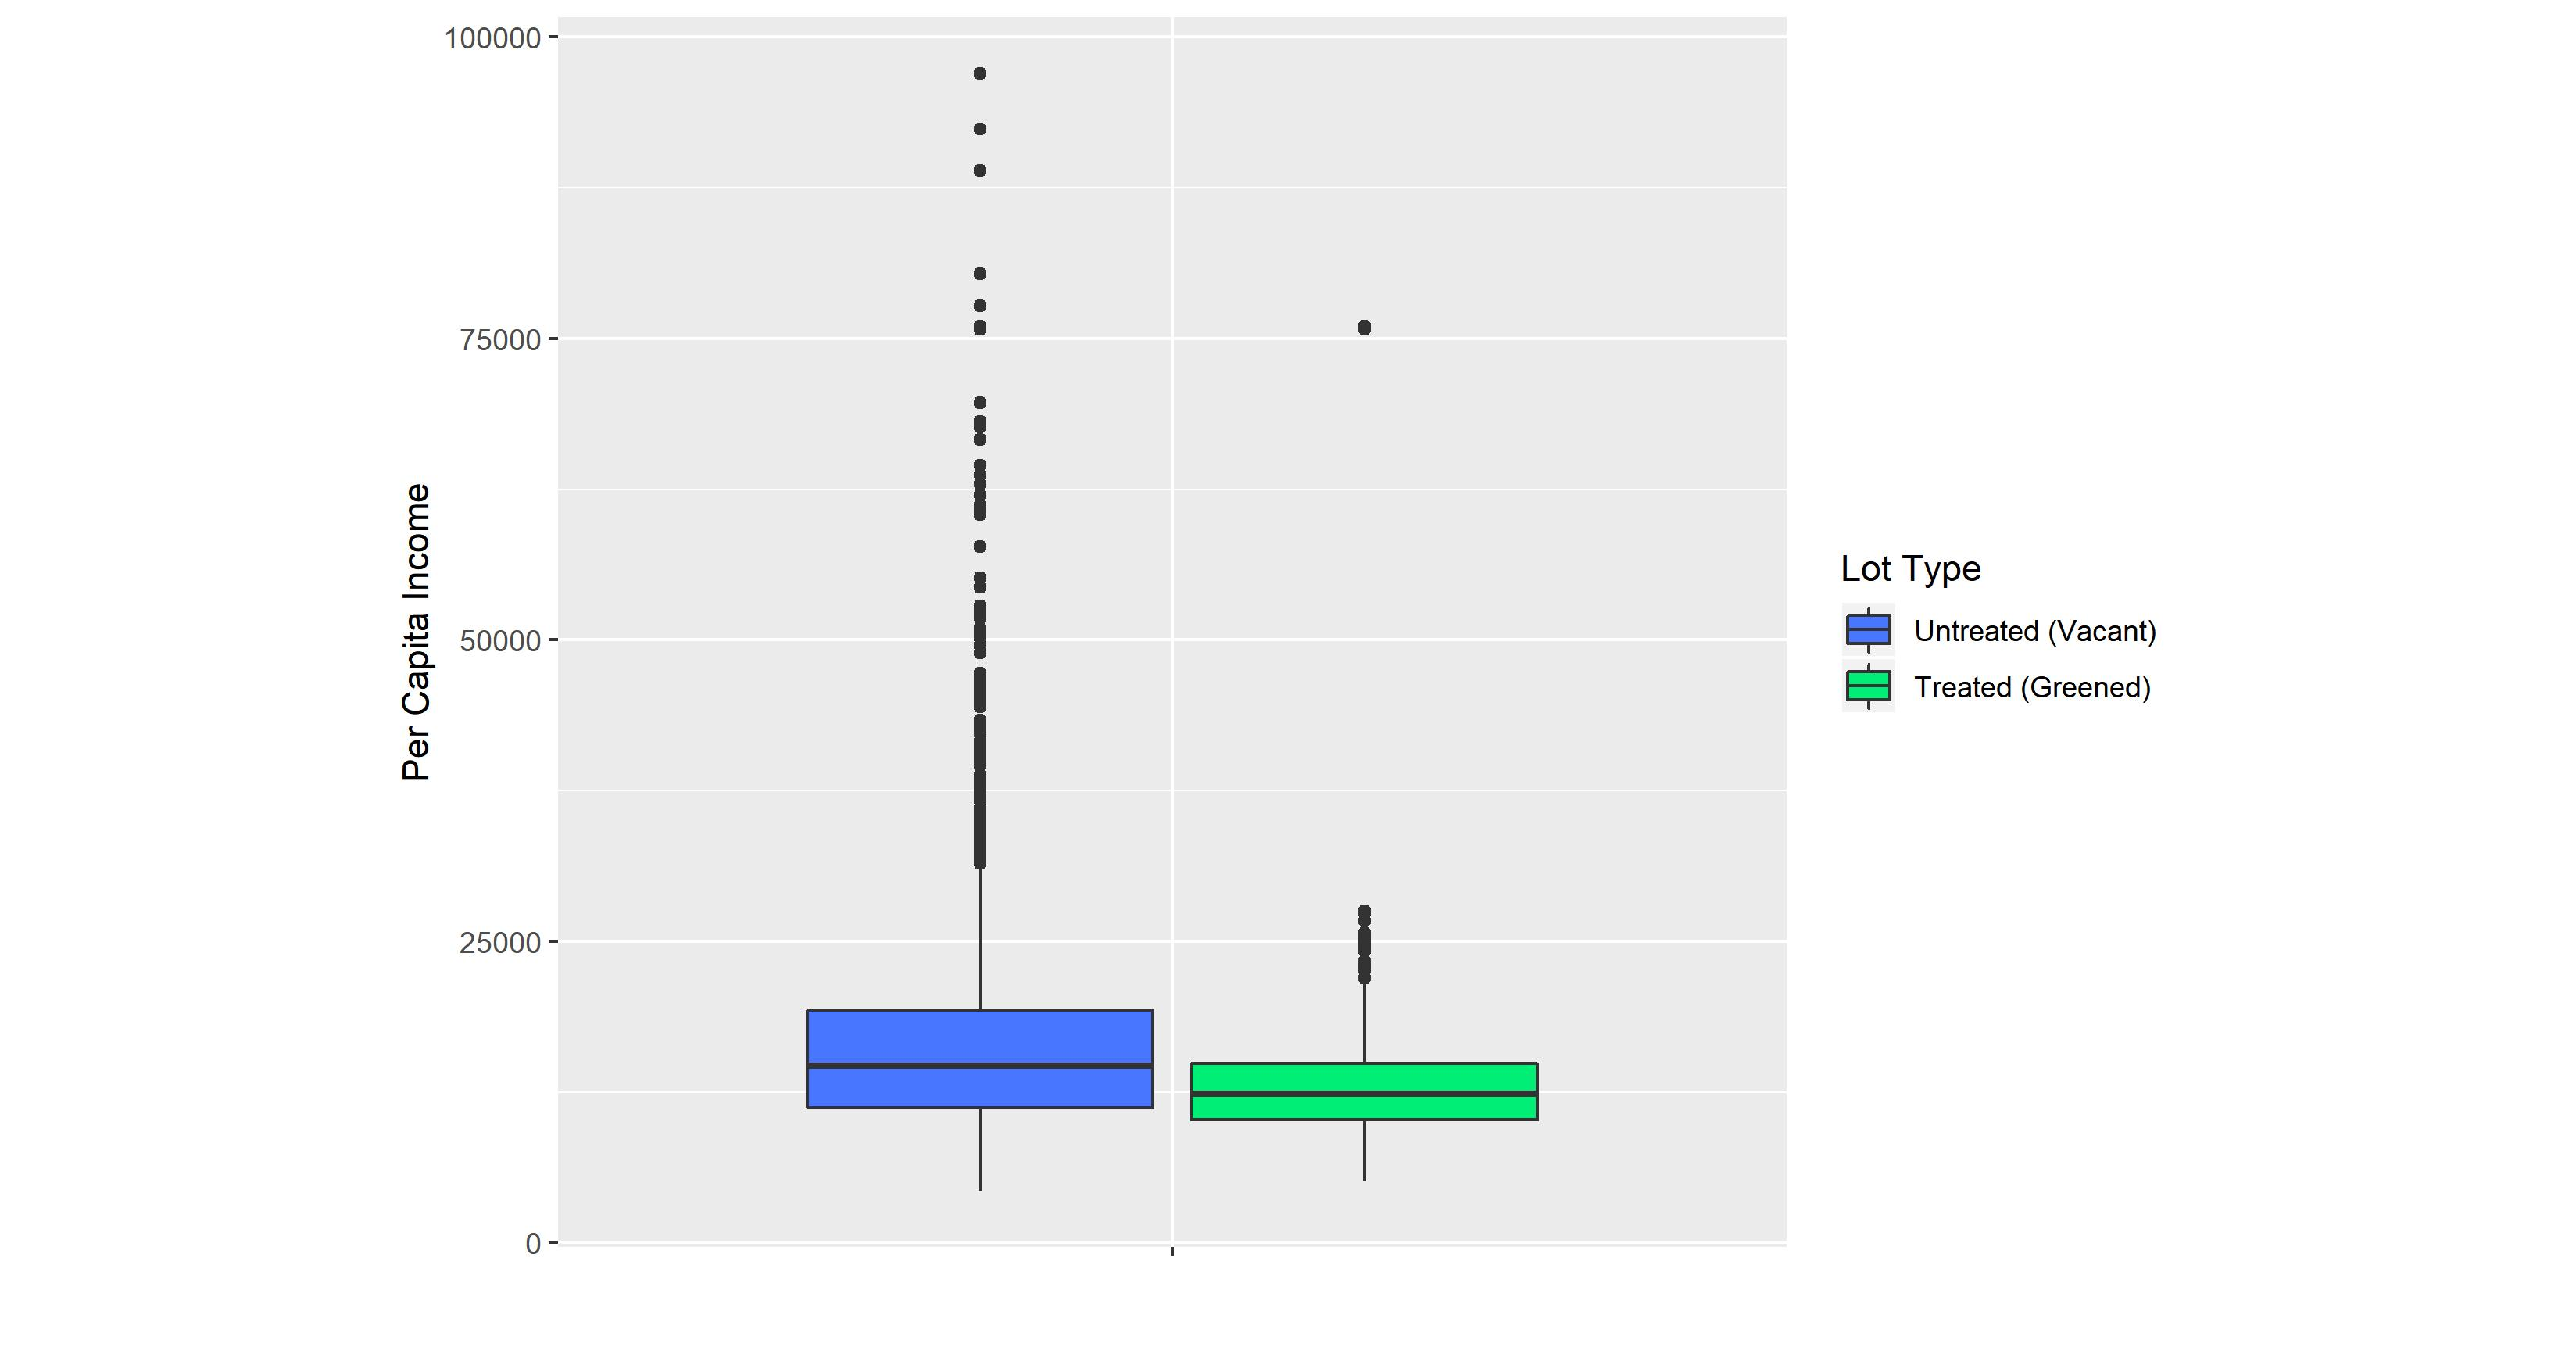
\includegraphics[width=10cm]{imgs/chart_pci.jpg}
    \centering
    \caption{Per capita income in 2015 adjusted inflation dollars for greened and non-greened lots}
    \label{fig:figure5}
    \end{figure}
    The data suggests that greened lots tend to occur in neighborhoods with lower per capita income, although the difference is small.    
    Figure \ref{fig:figure6} displays a box and whisker plot comparing poverty to income ratio brackets vacant lots without greening and greened lots.
    \begin{figure}[h]
    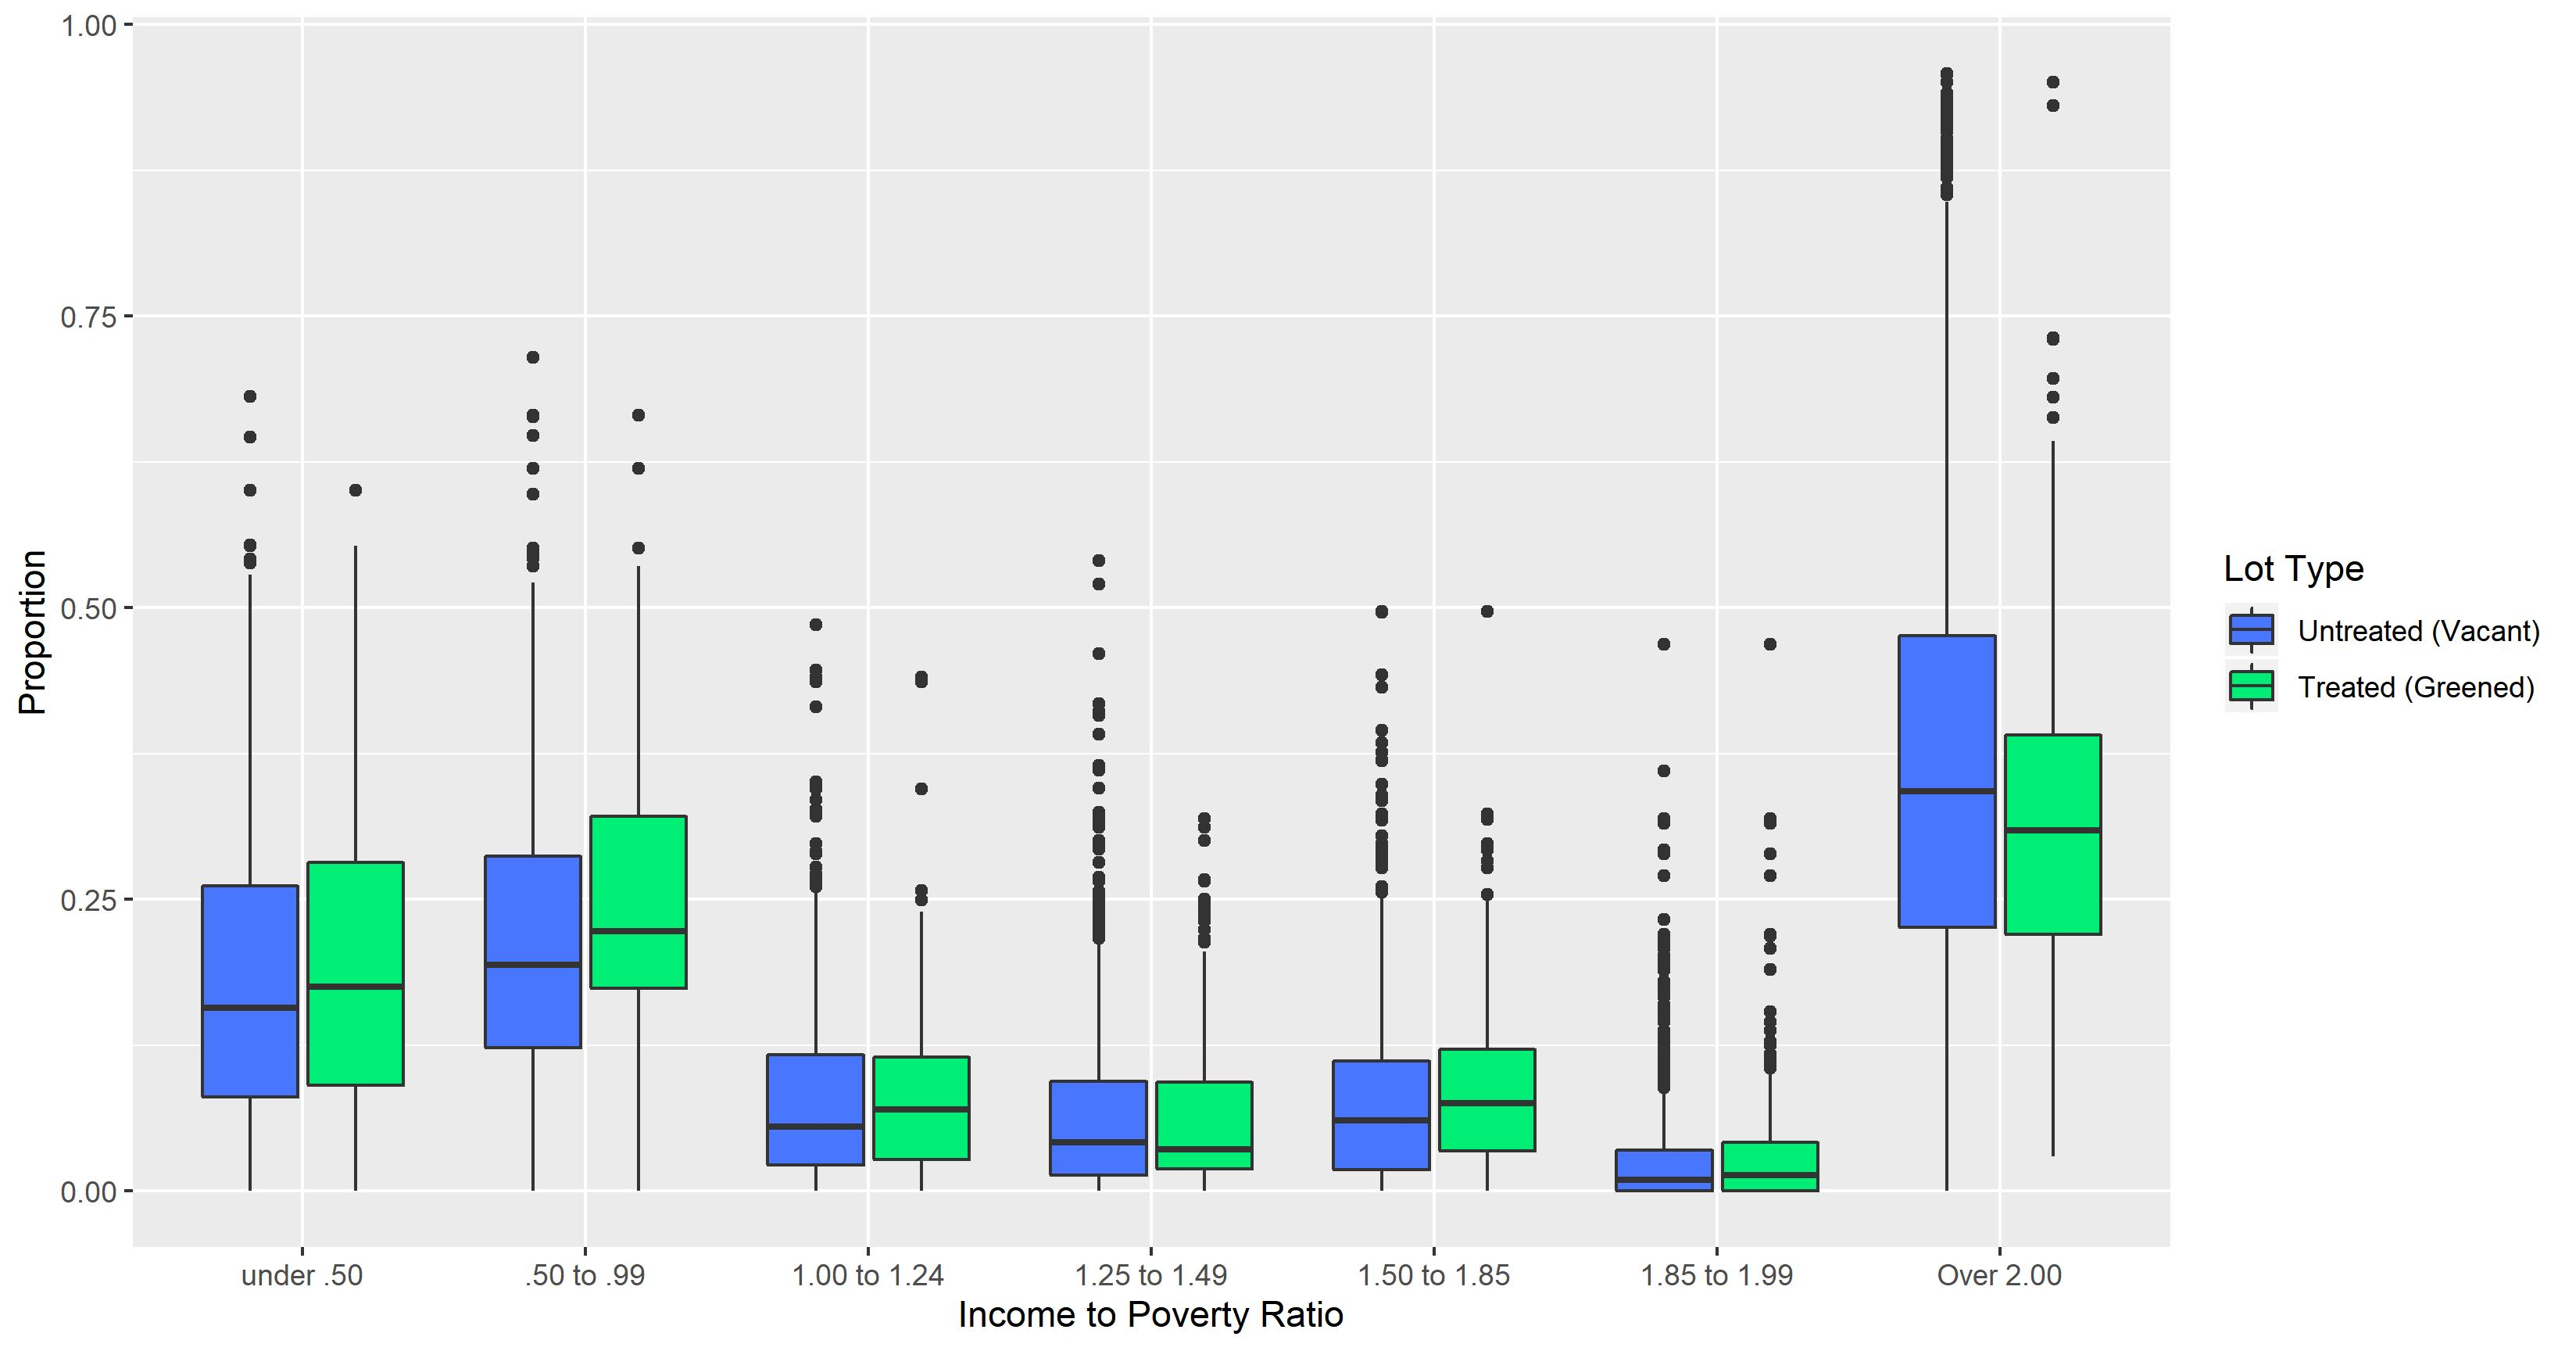
\includegraphics[width=10cm]{imgs/chart_inc_pov.jpg}
    \centering
    \caption{Income to poverty ratios in 2015 adjusted inflation dollars for greened and non-greened lots}
    \label{fig:figure6}
    \end{figure}
    When compared to vacant lots, we observe that treated greened lots are located in neighborhoods with lower income to poverty ratios, especially in brackets under 0.99 . They occur at a lower rate than vacant, non-treated lots in neighborhoods with extremely high income to poverty ratios over 2.00. The results on the economic health surrounding lots shown suggests that lots chosen to be treated and greened tend to be located in lower-income neighborhoods within Philadelphia. 
    \item \textbf{Land Use Zone Comparisons Between Lot Types} \\
    Figure \ref{fig:figure7} displays a box and whisker plot comparing land use proportions between vacant lots without greening and greened lots.
    \begin{figure}[h]
    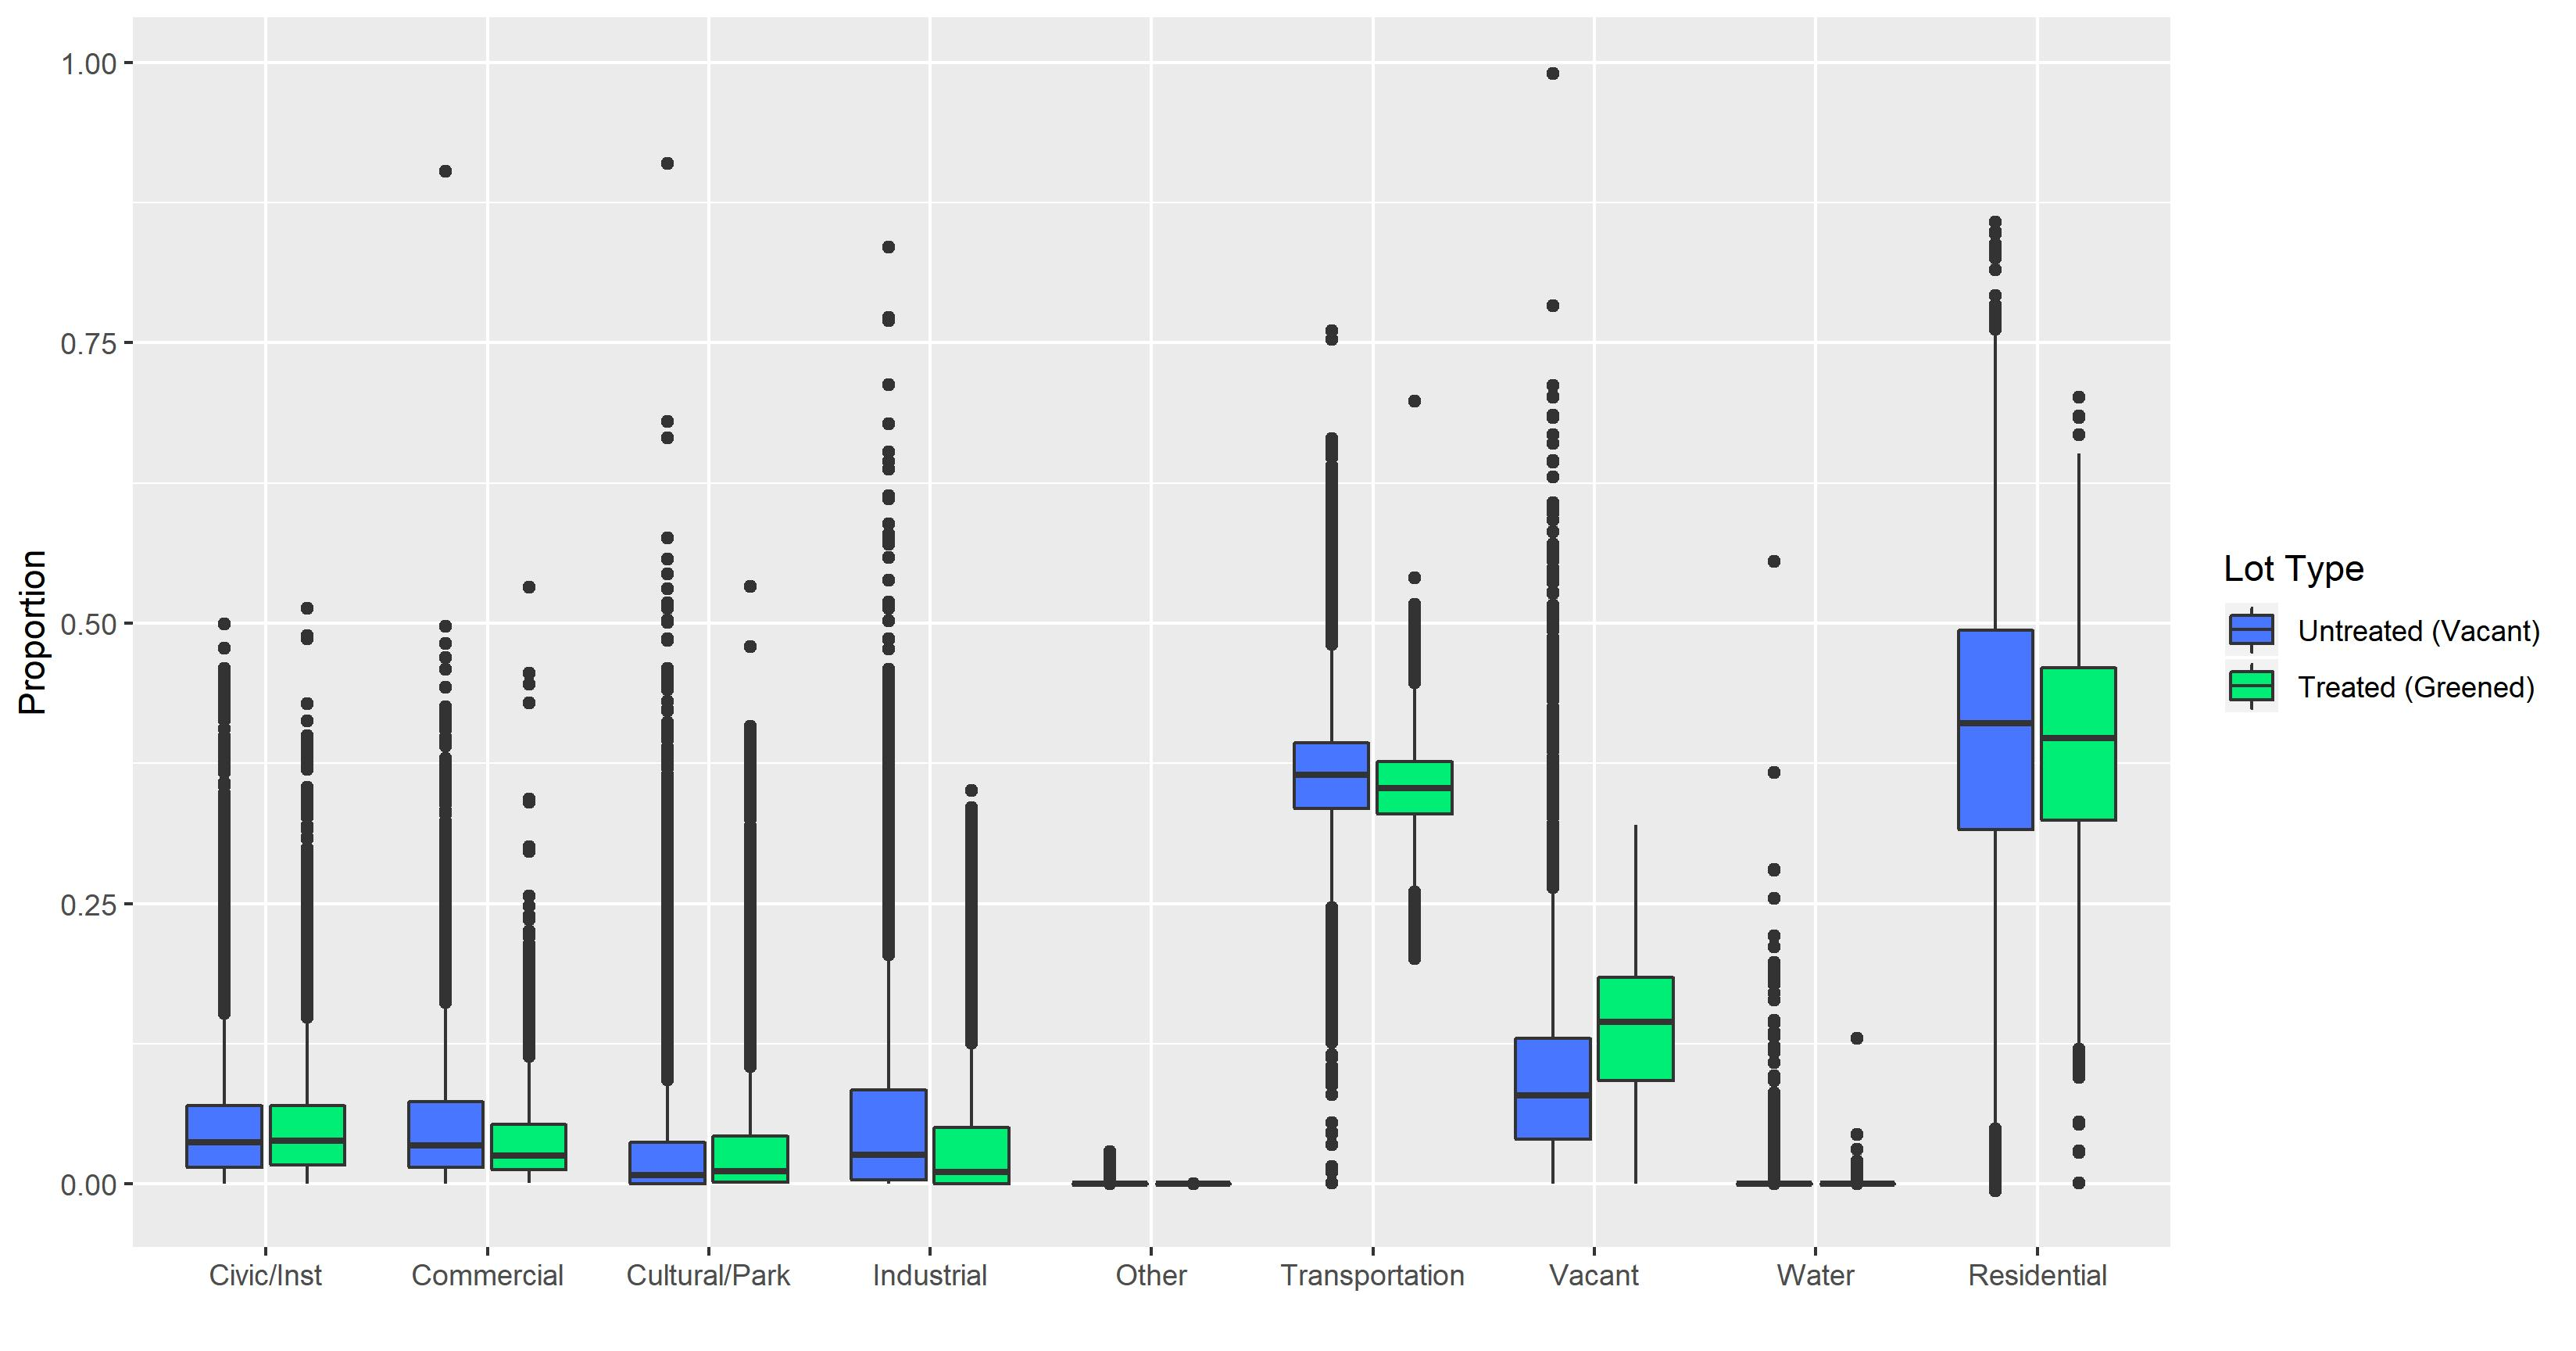
\includegraphics[width=12cm]{imgs/chart_land_use.jpg}
    \centering
    \caption{Land use proportions of greened and non-greened vacant lots}
    \label{fig:figure7}    
    \end{figure}
    In general, greened and non-greened lots have approximately equal land use proportions. Minor differences include how treated lots occur in neighborhoods with less commercial and industrial zones, but more in cultural/park zones. Lots are also chosen to be greened consistently in areas with moderate transportation land use. The variance of transportation land use in greened lots is smaller than the variance of transportation land use in vacant lots. We also observe that greened lots occur in regions with a higher proportion of vacant land use than non-greened lots.
    
     \item \textbf{Business Vibrancy Comparisons Between Lot Types} \\
    Figure \ref{fig:figure8} displays a box and whisker plot comparing business counts in a 200 meter radius surrounding vacant lots without greening and greened lots.
    \begin{figure}[h]
    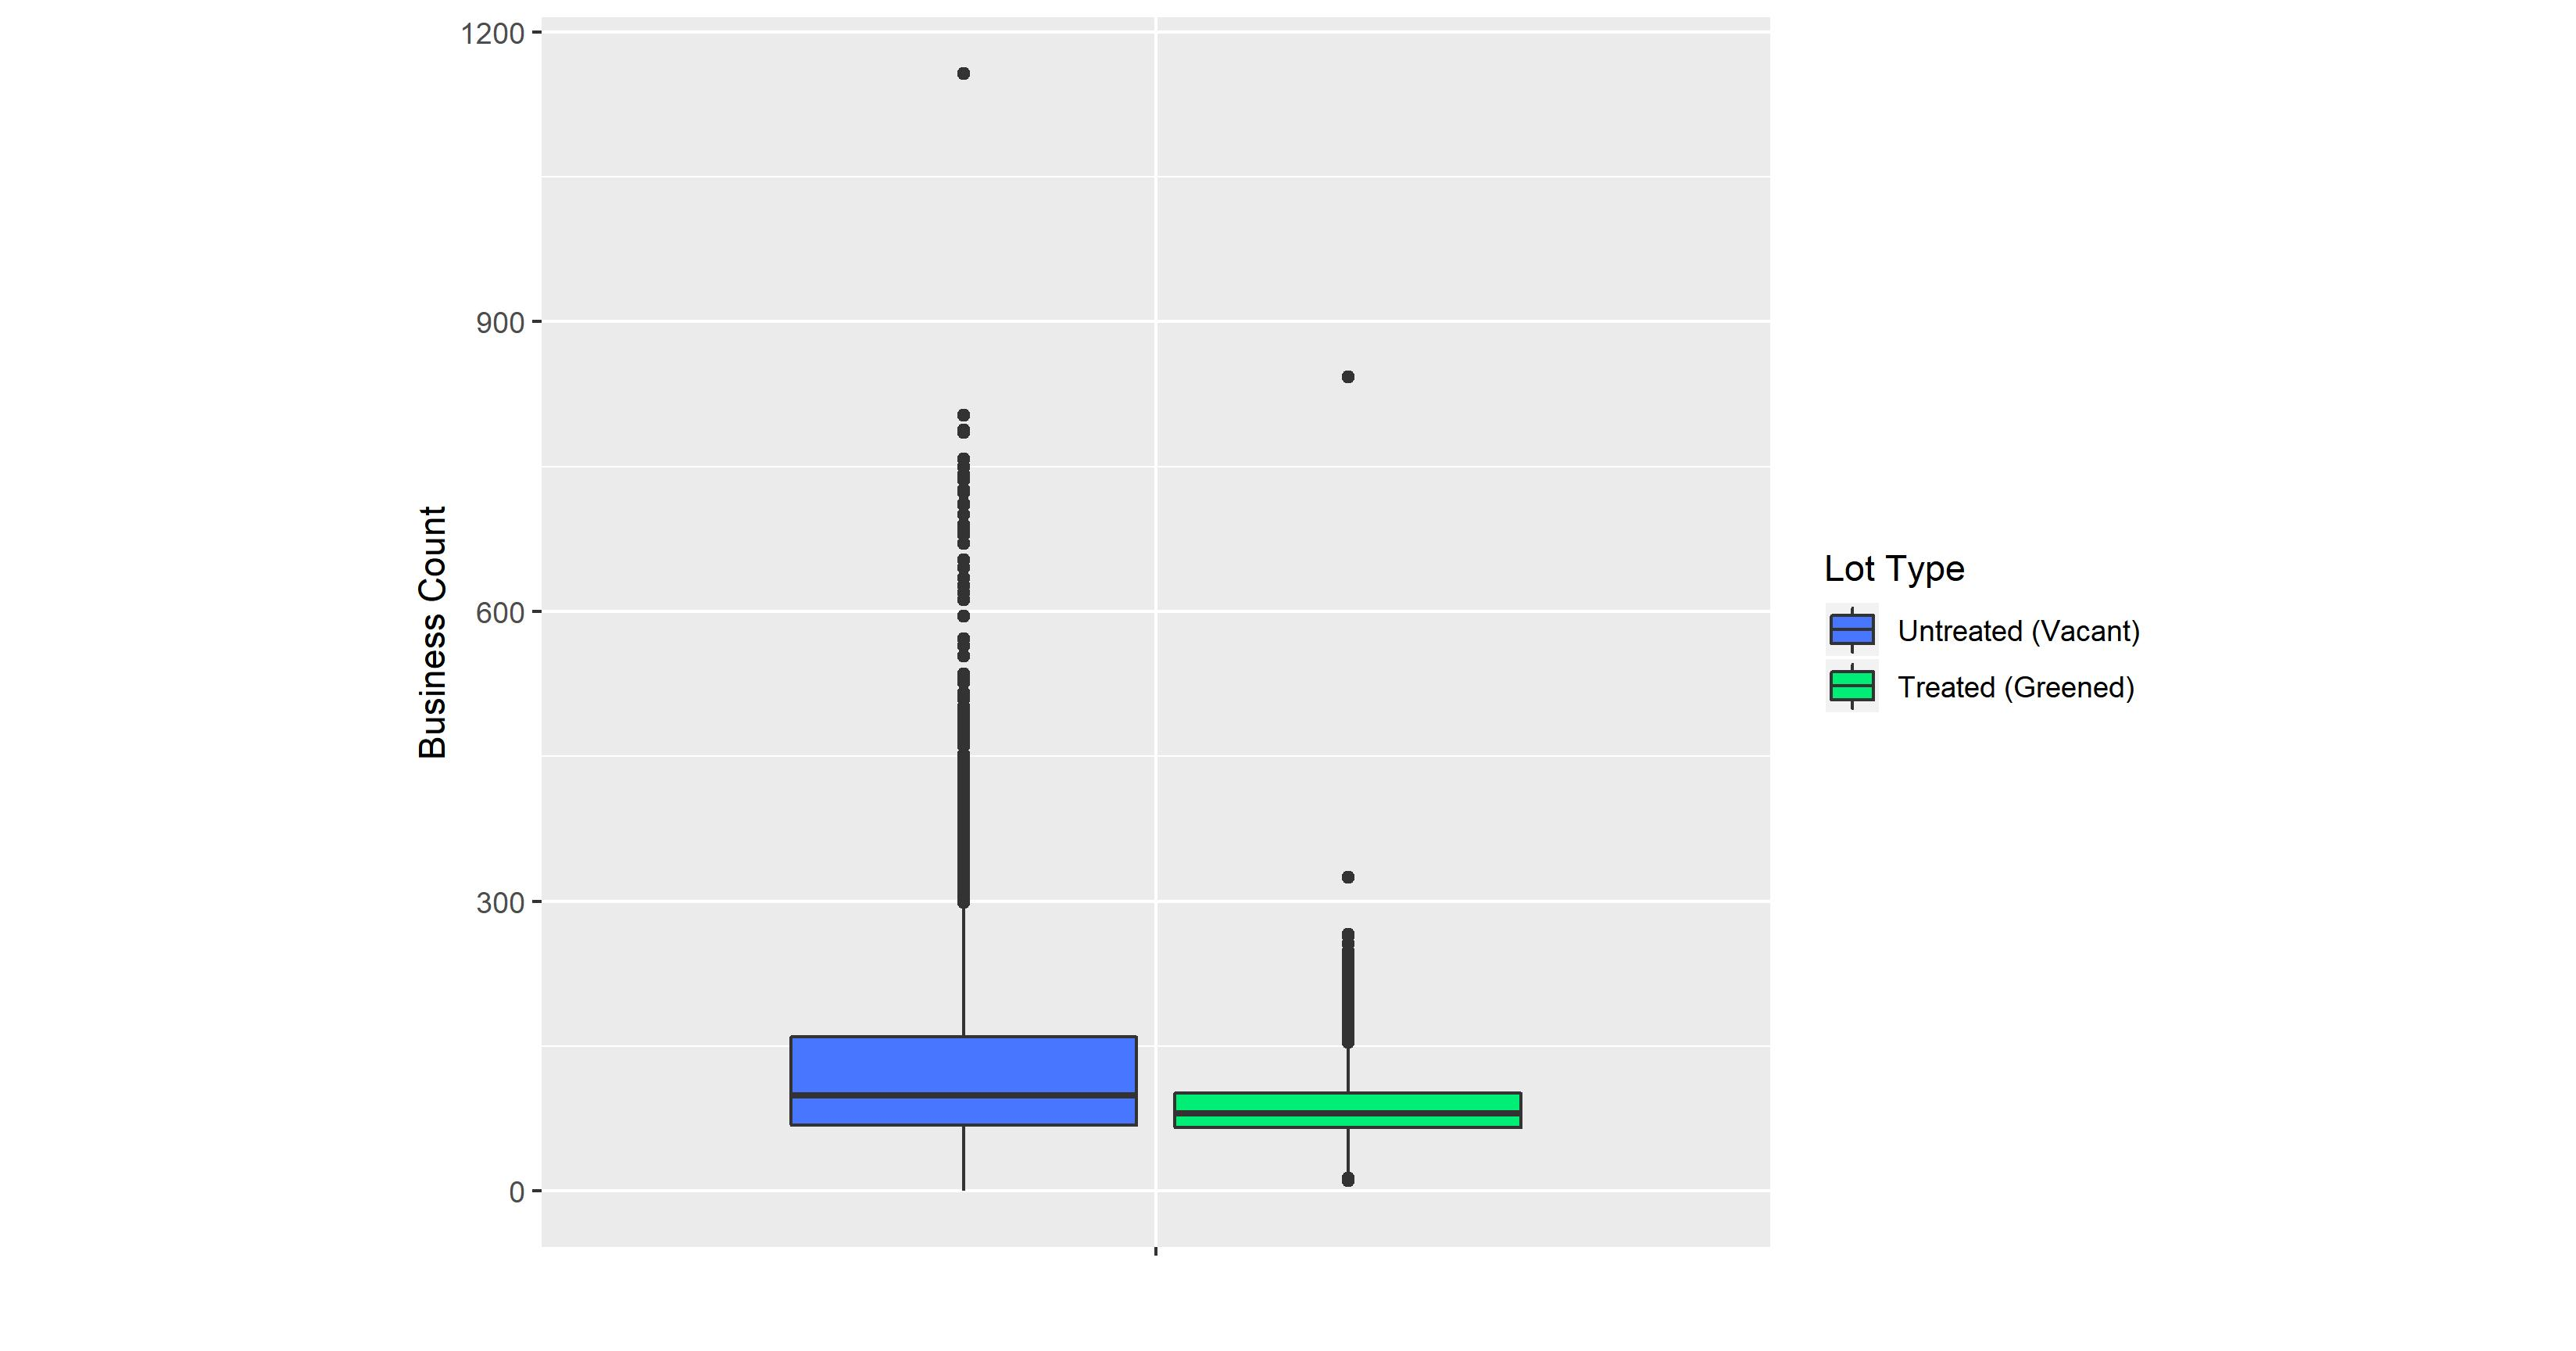
\includegraphics[width=10cm]{imgs/chart_bus_count.jpg}
    \centering
    \caption{Business counts of region surrounding of greened and non-greened vacant lots}
    \label{fig:figure8}
    \end{figure}
    We saw before that the region surrounding a treated lot has less commercial zoning compared to non-treated lots. Similarly, we see that the number of businesses surrounding treated lots is smaller than the number of businesses surrounding vacant lots.
    
    Figure \ref{fig:figure9} displays a graph highlighting the proportions of greened and vacant lots that contain a certain business type within a 200 meter radius.
    \begin{figure}[h]
    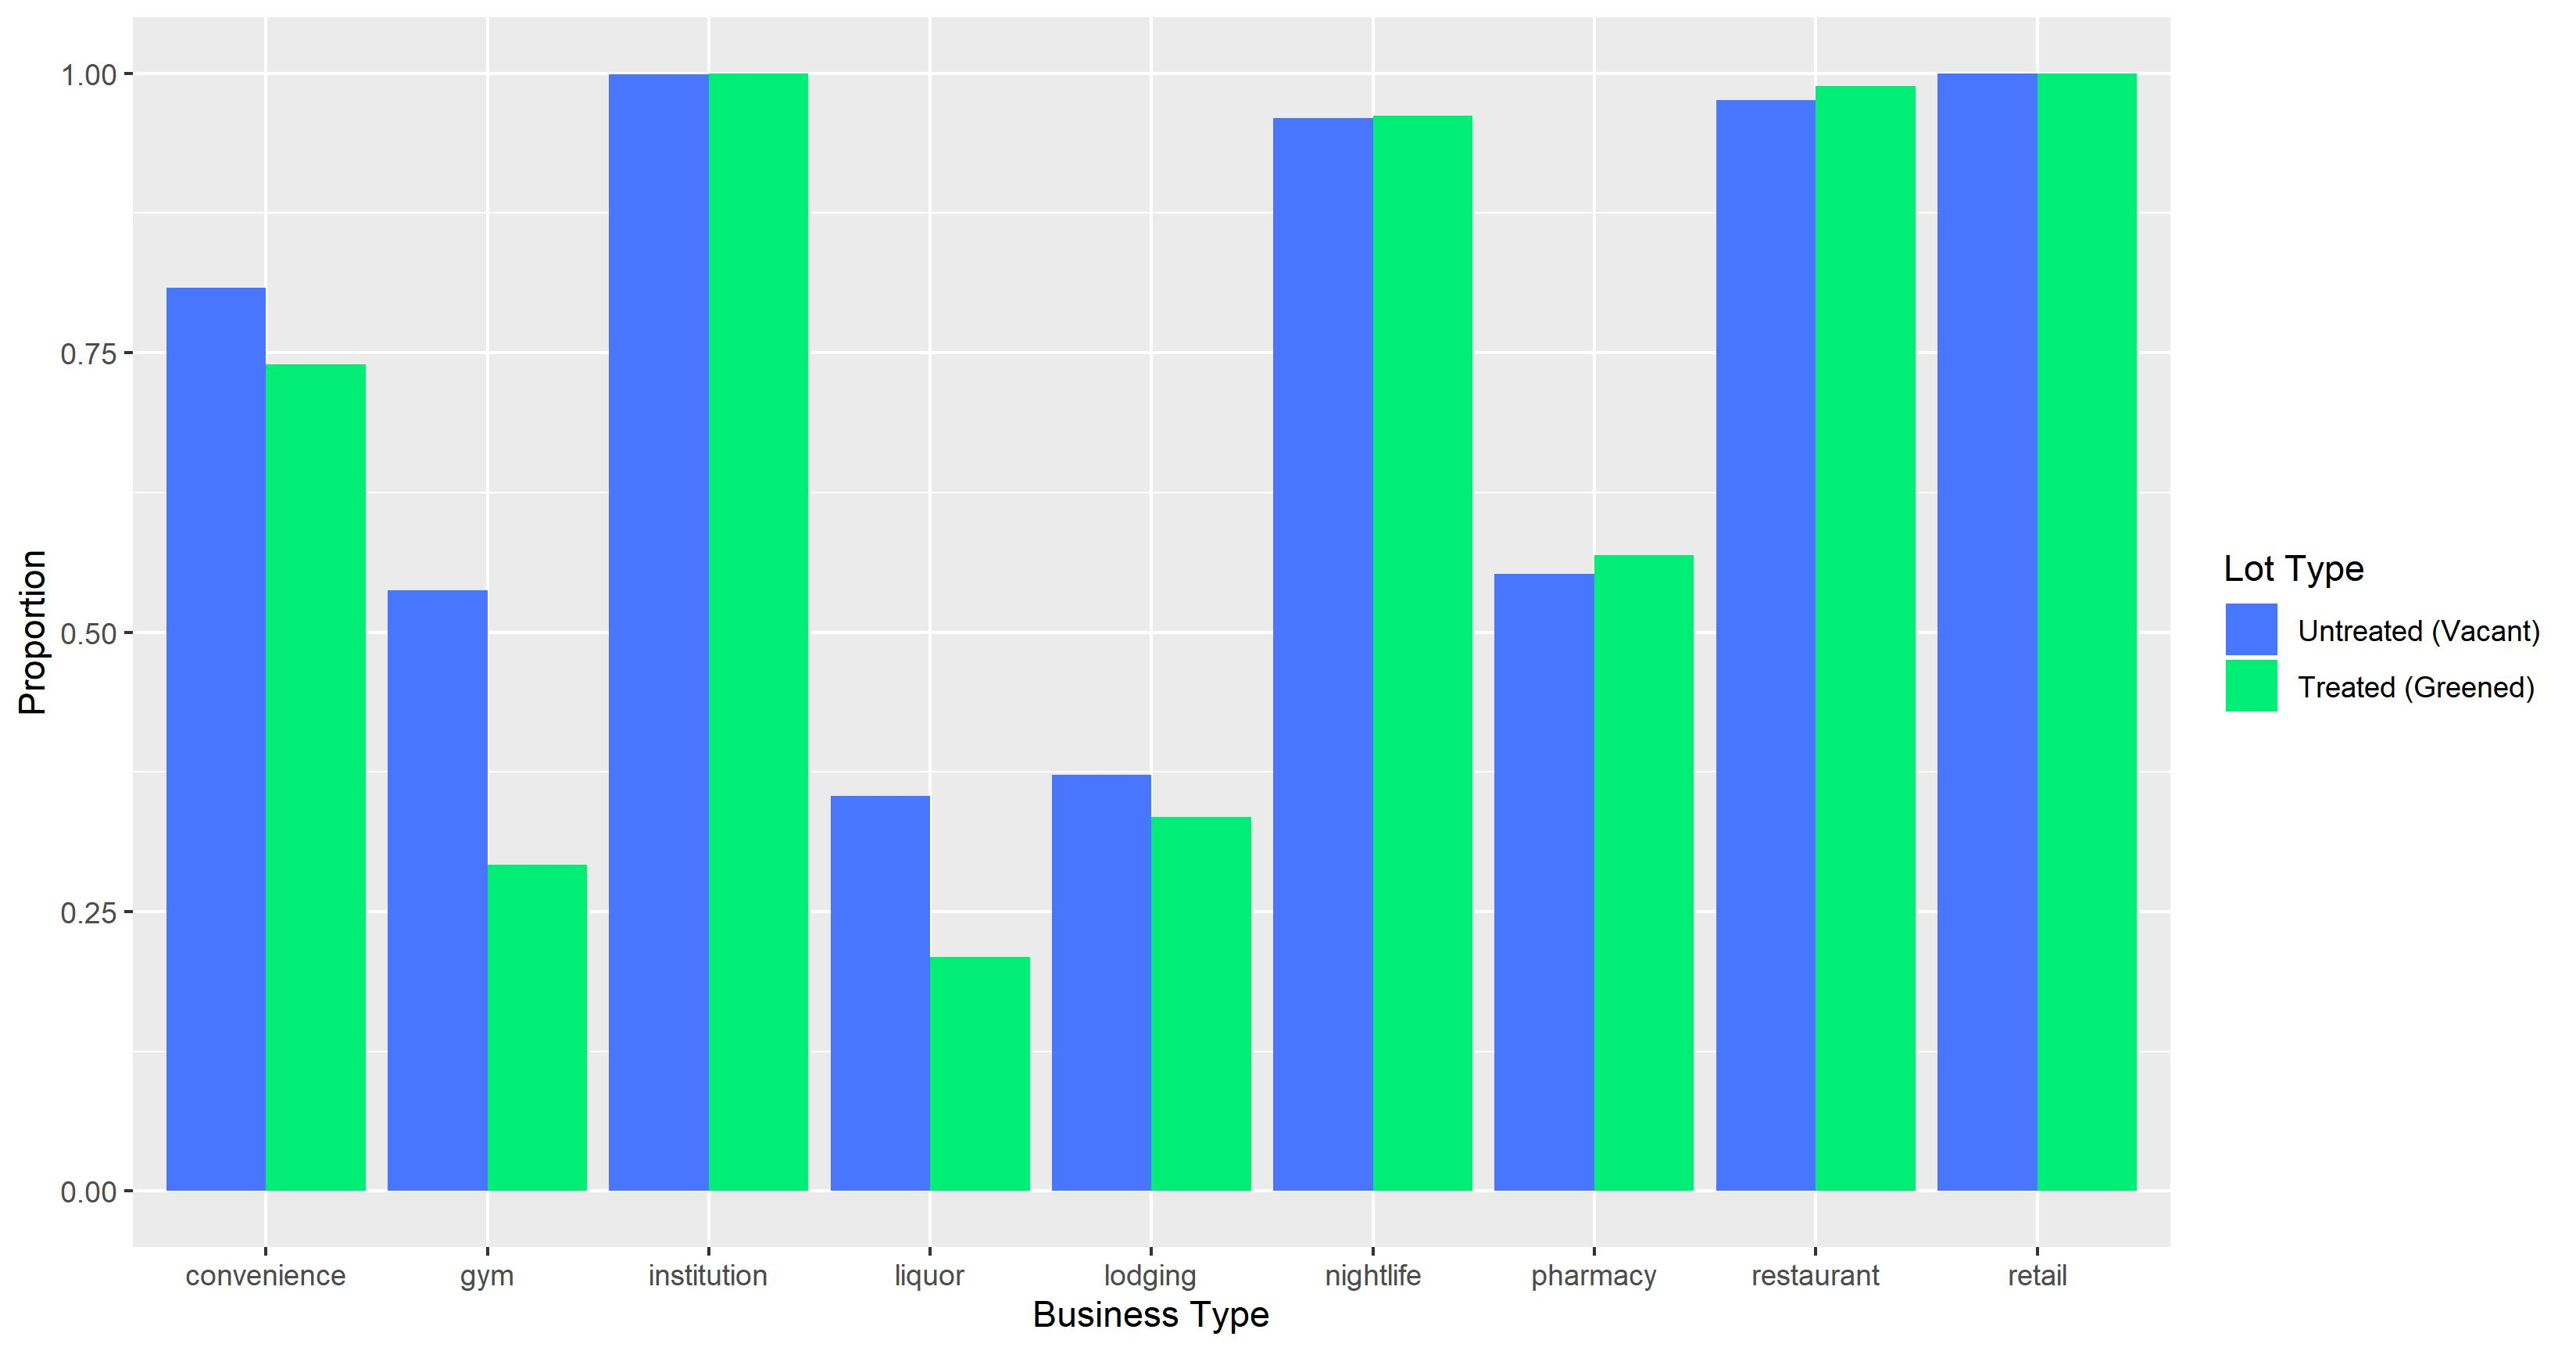
\includegraphics[width=10cm]{imgs/chart_bus_vib.jpg}
    \centering
    \caption{Business characteristics of region surrounding of greened and non-greened vacant lots}
    \label{fig:figure9}
    \end{figure}
    Both greened and vacant lot regions consistently contain institutions, nightlife, restaurants, and retail. Treated lot regions on average contain convenience stores, gyms, liquor stores, and lodging at a lower rate than non-treated vacant lots.
\end{enumerate}
\section{Creating Matched Pairs for Treated and Vacant Lots}
\subsection{Propensity Scoring and Matching}
As seen above, there are clear confounding variables and hidden biases if we choose to perform a simple means difference-in-differences test to determine whether greening intervention reduces crime counts. To reduce these biases, we instead opt for matched pairs testing, where we match a greened lot to a vacant lot with similar propensity to be treated as the greened lot, based on the characteristics of that lot and the region surrounding it. In this manner, we can also set our greening intervention date for our control vacant lots to be the same date as the intervention date of its paired green lot. This way, the test also controls for temporal biases. Essentially, we compare greened lots crime changes to the crime changes of vacant lots very similar to the greened lots. These vacant lots act as counterfactual observations to what would have occurred had there been no greening. We will then perform a matched pairs t-test to get a more accurate calculation of the crime difference-in-differences between greened and vacant lots before and after intervention. 

We created propensity scores for all of our lots based on their propensity to be greened using a logistic regression model. Out of the variables involving land use zoning, we removed the “Other” category and the income to poverty ratio above 2.00 bracket to account for collinearity. We then dropped the institution and retail business vibrancy categories from our dataset since almost all of the calculated lot regions contained at least one of these businesses leading to singularity errors in our regression. The presence of these business types are not differentiated among different lots and so they are excluded from the propensity scores.

We fitted a general logistic regression model onto our covariates. The coefficients support the general differences between greened and vacant lots that we discussed in the previous section.

We also observed the effects of individual covariates in the sections of economic, demographic, land use, and business vibrancy to see how helpful variables in each category are to the propensity model shown in table \ref{tab:perfm}. For accuracy metrics, we chose the decision boundary for our logistic regression model to be at the percent of all lots in our dataset that is greened. This number is $\frac{n_{greened}}{n_{total}} = \frac{4651}{21425} = 0.2170828$. Anything above this decision boundary would have been predicted as a greened lot.

\begin{table}[H]
\begin{center}
\caption{\label{tab:perfm}Performance Metric of Logistic Models by Feature Group}
\begin{tabular}{@{}llllll@{}}
\toprule
\textbf{Metric}               & \textbf{Overall} & \textbf{Economic} & \textbf{Demographic} & \textbf{Land Use} & \textbf{Business} \\ \midrule
\textbf{ROC AUC}              & 0.81060          & 0.66308           & 0.70599              & 0.74170           & 0.67408           \\
\textbf{Accuracy}             & 0.71496          & 0.60761           & 0.59239              & 0.67594           & 0.61274           \\
\textbf{Balanced Accuracy}    & 0.74151          & 0.62688           & 0.64738              & 0.68108           & 0.64375           \\
\textbf{Kappa}                & 0.36549          & 0.18021           & 0.19731              & 0.27530           & 0.20151           \\
\textbf{Sensitivity}          & 0.69459          & 0.59282           & 0.55020              & 0.67199           & 0.58895           \\
\textbf{Specificity}          & 0.78843          & 0.66093           & 0.74457              & 0.69017           & 0.69856           \\
\textbf{Pos Pred Value}       & 0.92212          & 0.86312           & 0.88596              & 0.88665           & 0.87572           \\
\textbf{Neg Pred Value}       & 0.41718          & 0.31038           & 0.31459              & 0.36846           & 0.32029           \\
 \bottomrule
\end{tabular}
\end{center}
\end{table}

We observe that demographic, economic, and land use variables each individually influence the logistic regression model in a predictive manner. The model with all variables performs the best with balanced accuracy and other metrics. Out of all the sub-categories of covariates, land use is the most predictive in terms of ROC AUC and balanced accuracy on whether a lot is greened, followed by demographic variables, business variables, and lastly economic variables. As can be observed, each logistic model by category performs slightly better than guessing rate when using balanced accuracy as the metric, and the combination of all these features from all groups provides us with the model with the best balanced accuracy.

We also plotted the ROC (Receiving Operating Characteristic) curves for each of the covariate groups shown in Figure \ref{fig:figure10}. The model using all covariates has the most superior ROC as seen in the chart, followed by the model using land use covariates. 

\begin{figure}[h]
    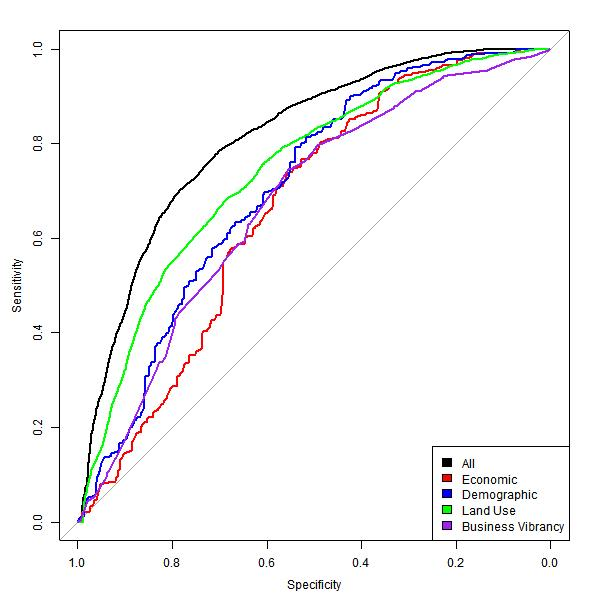
\includegraphics[width=6cm]{imgs/rocs.jpg}
    \centering
    \caption{ROC Curves for Different Covariate Groups Predicting Greening in Lots}
    \label{fig:figure10}
\end{figure}


\subsection{Matched pairs and covariate balancing}
Using the propensities calculated from the logistic model on all variables as the distance metric, we matched control vacant lots to treated greened lots by nearest neighbor matching. We were able to match all treated lots to one control lot each. We used Mahalanobis distance matching on all the covariates with a 0.2 caliper. 

We ran two sets of matching. One without business vibrancy characteristics, and one with business vibrancy characteristics. The resulting effect of the propensity score matching of units on all covariates can be observed with the covariate balance chart on figure \ref{fig:a}. The propensity scoring shows significant covariate balancing. All covariates are within 0.2 absolute standardized mean differences from each other after balancing for both matching with business vibrancy characteristics and matching without.

 \begin{figure}[h]
    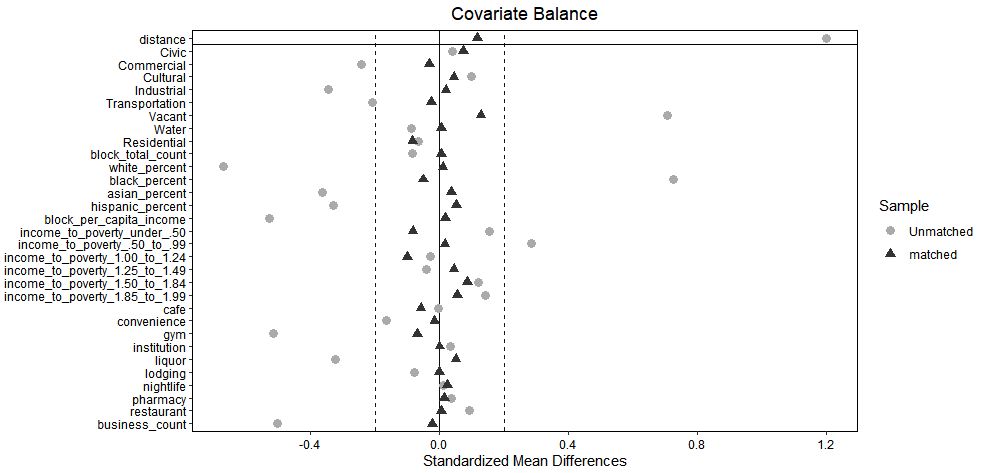
\includegraphics[width=8cm]{imgs/propensity_balance.png}
    \centering
    \caption{\label{fig:a}Covariate Balancing After Propensity Score Matching}
\end{figure}

\section{Analysis and Discussion of Results}
\subsection{General Matched Pairs t-tests}
We ran matched-pairs t-tests on each of the three radius categories and nonviolent, violent, and total crimes. The results for t-tests without propensity scoring and matching on business vibrancy characteristics are shown in table \ref{tab:g}. Displayed in table \ref{tab:h} are the results for t-tests with propensity scoring and matching on business vibrancy characteristics.
\begin{table}[h]
\begin{center}
\caption{\label{tab:g}Matched pairs t-tests on demographic, economic, and land use features}
\begin{tabular}{lllllll}
\hline
\textbf{t} & \textbf{p} & \textbf{est} & \textbf{se} & \textbf{dof} & \textbf{type}       & \textbf{radius} \\ \hline
-6.16501   & 7.67E-10   & -2.34769     & 0.380809    & 4434         & total      & 100    \\
-3.69467   & 0.000223   & -3.05727     & 0.827483    & 4434         & total      & 200    \\
-9.85415   & 1.12E-22   & -21.2891     & 2.160416    & 4434         & total      & 500    \\
-5.85928   & 4.99E-09   & -1.89605     & 0.323598    & 4434         & nonviolent & 100    \\
-3.7344    & 0.000191   & -2.72717     & 0.730284    & 4434         & nonviolent & 200    \\
-10.3035   & 1.29E-24   & -20.639      & 2.003116    & 4434         & nonviolent & 500    \\
-3.45344   & 0.000559   & -0.45163     & 0.130778    & 4434         & violent    & 100    \\
-1.37328   & 0.169734   & -0.3301      & 0.240374    & 4434         & violent    & 200    \\
-1.17237   & 0.241111   & -0.65006     & 0.55448     & 4434         & violent    & 500    \\ \hline
\end{tabular}
\end{center}
\end{table}

\begin{table}[h]
\begin{center}
\caption{\label{tab:h}Matched pairs t-tests on demographic, economic, and land use features}
\begin{tabular}{lllllll}
\hline
\textbf{t} & \textbf{p} & \textbf{est} & \textbf{se} & \textbf{dof} & \textbf{type}       & \textbf{radius} \\ \hline
-6.0736    & 1.36E-09   & -2.34965     & 0.386863    & 4329         & total         & 100             \\
-5.57598   & 2.61E-08   & -4.57206     & 0.819956    & 4329         & total         & 200             \\
-12.1479   & 2.05E-33   & -26.5159     & 2.18276     & 4329         & total         & 500             \\
-5.76275   & 8.85E-09   & -1.86998     & 0.324494    & 4329         & nonviolent    & 100             \\
-5.61113   & 2.14E-08   & -4.02494     & 0.717314    & 4329         & nonviolent    & 200             \\
-13.2536   & 2.49E-39   & -26.4764     & 1.997681    & 4329         & nonviolent    & 500             \\
-3.57723   & 0.000351   & -0.47968     & 0.134092    & 4329         & violent       & 100             \\
-2.24899   & 0.024563   & -0.54711     & 0.243271    & 4329         & violent       & 200             \\
-0.0708    & 0.943564   & -0.03949     & 0.557835    & 4329         & violent       & 500             \\ \hline
\end{tabular}
\end{center}
\end{table}
The results show that for total crimes in all radii tested, greening intervention on vacant lots significantly reduces the amount of crimes in an area. For total and nonviolent crimes, the effects of greening scale with and are significant with increasing radii up to and including 500 meters. For violent crimes, the effects of greening scale off with increasing radii and do not become significant after 200 meters for without matching on business vibrancy and after 500m for with controlling for business vibrancy.
\subsection{Influences of Land Use Zoning on Tests}
We then wanted to observe the effect of individual neighborhood area characteristics, in particular land use zoning and business vibrancy, on the effects of greening. In other words, we asked ourselves questions such as does the existence of a cafe in a neighborhood decrease crime rates further after the intervention of vacant lot greening in that neighborhood?

To do so, we grouped our data into various subsets. For each continuous feature, we performed t-tests with all the pairs with feature values under the 25th percentile and all the pairs with feature values over the 75th percentile of that feature. For each discrete binary variable, such as the business characteristics indicator variables, we performed t-tests individually on lot pairs each where both lots do not have the feature and lot pairs that both do have the feature.

We created a plot to illustrate how individual land use characteristics influence the effect of greening on crime shown in Figure \ref{fig:figure12}. The vertical line in the plot represents the average effect for all lots.

\begin{figure}[h]
    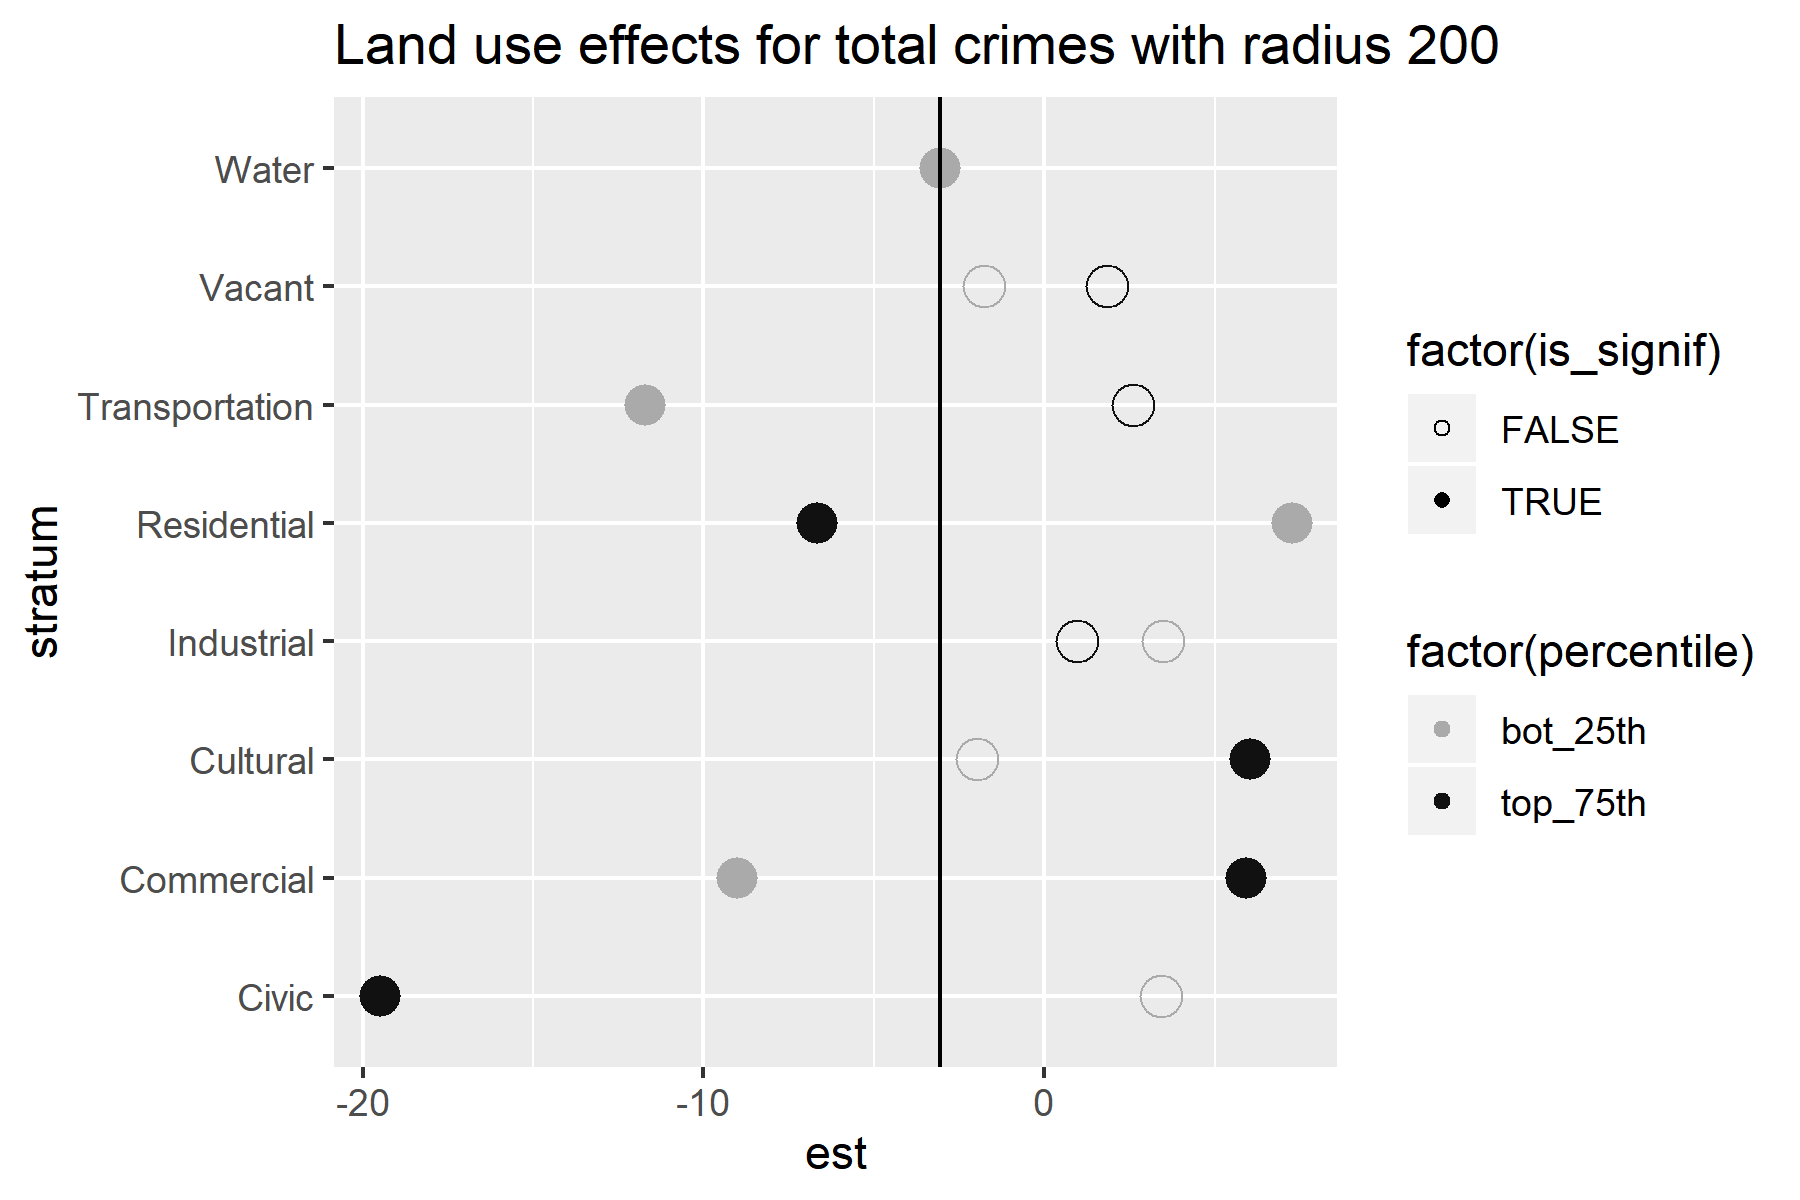
\includegraphics[width=8cm]{imgs/land_use_stratum_total_200.png}
    \centering
    \caption{Land Use Zoning Influences on Crime Effects of Greening Intervention}    
    \label{fig:figure12}
\end{figure}

The results of subsetting matched-pairs t-tests by high or low amounts of certain land-use zones show that certain land use zones do influence the crime effects of greening intervention.

Certain areas have a positive impact by further decreasing crimes within a 200 meter radius. 
\begin{itemize}
    \item Greening in \textbf{high residential areas} has a positive influence on decreasing crime further significantly for total, non-violent, and violent crimes (\textbf{118\% decrease} compared to average crime effect for total crimes at 200 meters). 
    \item Greening in \textbf{high civic/institution areas} has a positive influence on decreasing crime further significantly for total, non-violent, and violent crimes (\textbf{538\% decrease} compared to average crime effect for total crimes at 200 meters).
    \item Greening in \textbf{low transportation areas} has a positive influence on decreasing crime further significantly for total, non-violent, and violent crimes (\textbf{238\% decrease} compared to average crime effect for total crimes at 200 meters).
    \item Greening in \textbf{low commercial areas} has a positive influence on decreasing crime further significantly for total, non-violent, and violent crimes (\textbf{195\% decrease} compared to average crime effect for total crimes at 200 meters).
\end{itemize}


Greening in other areas has a negative impact on decreasing crimes within a 200 meter radius. 
\begin{itemize}
    \item Greening in \textbf{high cultural areas} has a negative influence on decreasing crime further significantly for total and nonviolent crimes (\textbf{298\% increase} compared to average crime effect for total crimes at 200 meters).
    \item Greening in \textbf{high commercial areas} has a negative influence on decreasing crime significantly for total, non-violent, and violent crimes (\textbf{293\% increase} compared to average crime effect for total crimes at 200 meters). 
    \item Greening in \textbf{low residential areas} has a negative influence on decreasing crime further significantly for total and nonviolent crimes (\textbf{338\% increase} compared to average crime effect for total crimes at 200 meters).
\end{itemize}

\subsection{Influences of Business Vibrancy on Tests}
Figure \ref{fig:figure13} results for individual tests on each business vibrancy characteristic. The vertical line in the plot represents the average effect for all lots.
\begin{figure}[h]
    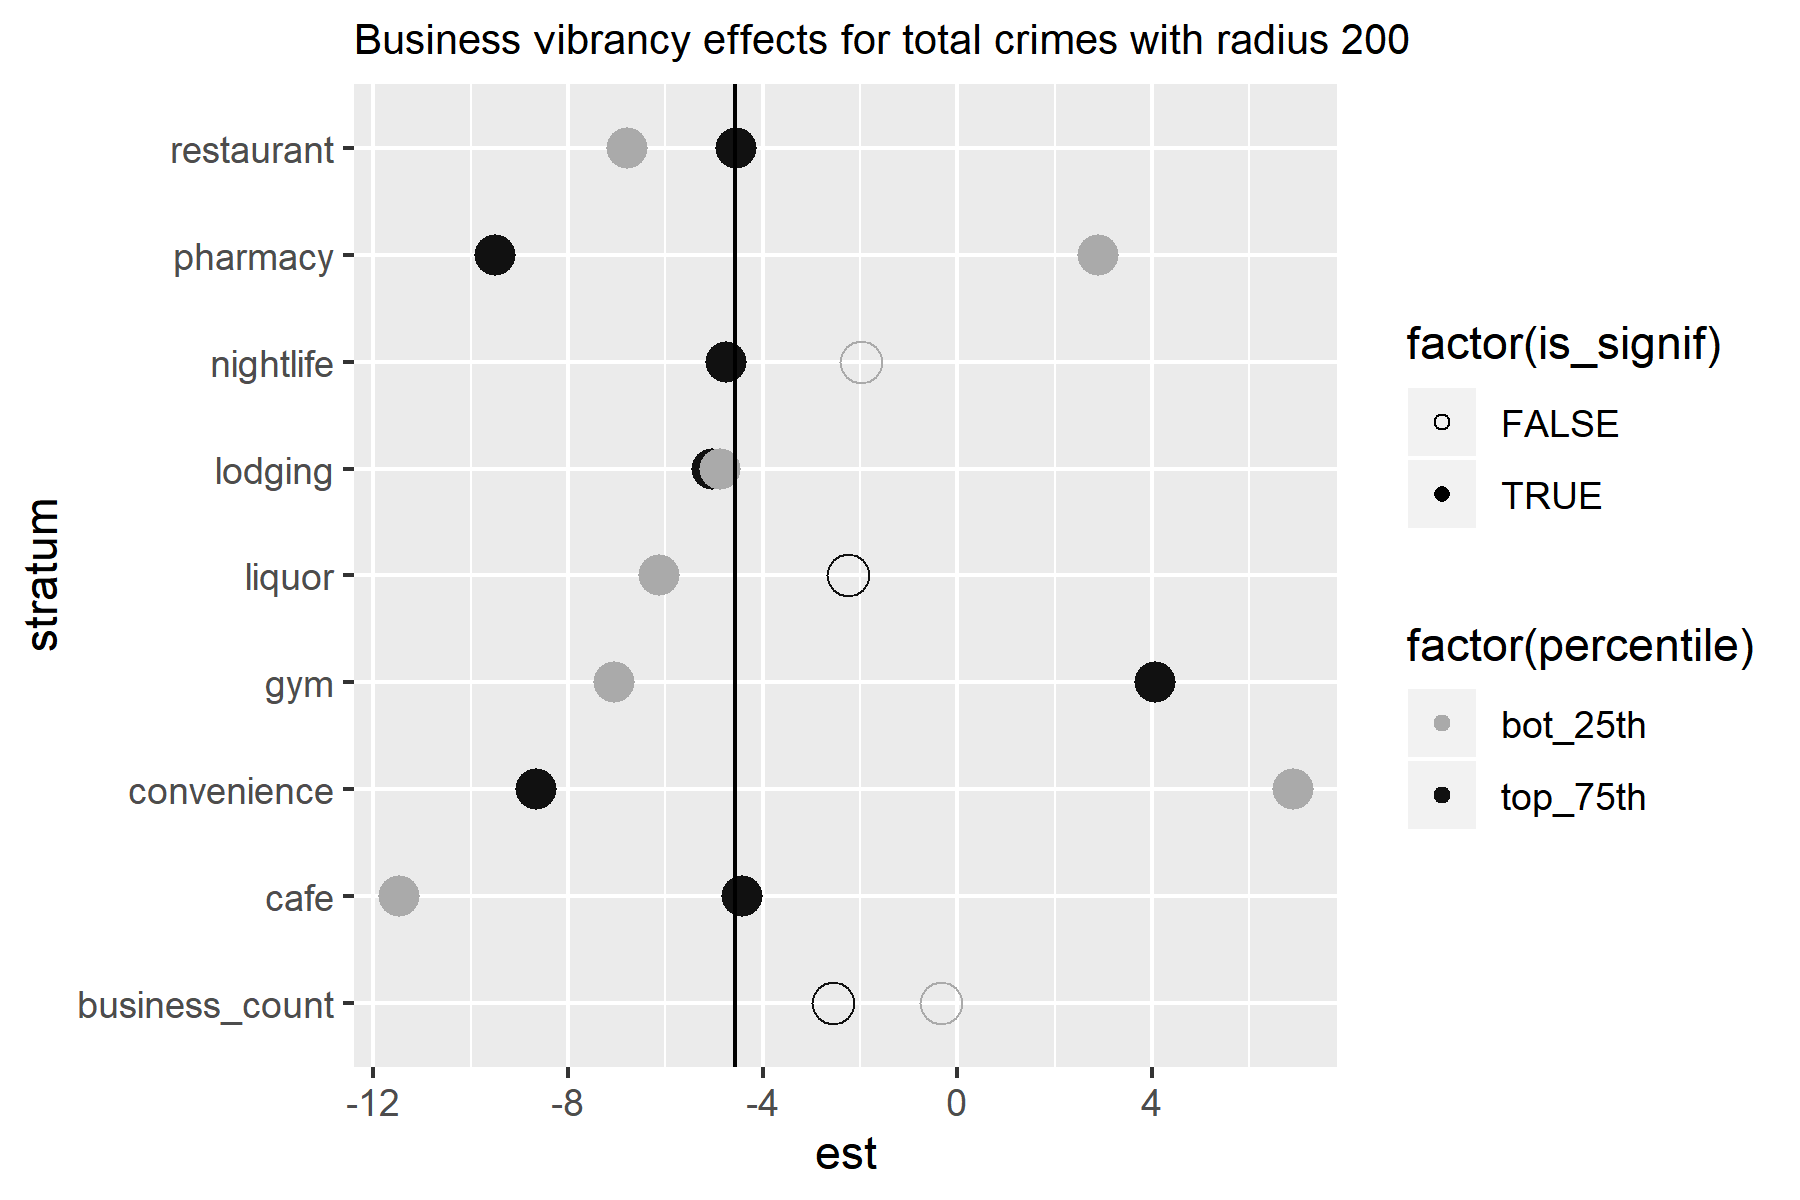
\includegraphics[width=10cm]{imgs/business_use_stratum_total_200.png}
    \centering
    \caption{Business Vibrancy Influences on Crime Effects of Greening Intervention}
    \label{fig:figure13}
\end{figure}
The results show that certain business vibrancy characteristics have a positive improvement on crime decrease within a 200 meter radius.
\begin{itemize}
    \item Greening in \textbf{areas with convenience stores} has a positive influence on decreasing crime further significantly for total, non-violent, and violent crimes (\textbf{89\% decrease} compared to average crime effect for total crimes at 200 meters).
    \item Greening in \textbf{areas with pharmacies} has a positive influence on decreasing crime further significantly for total and non-violent crimes (\textbf{108\% decrease} compared to average crime effect for total crimes at 200 meters).
    \item Greening in \textbf{areas without cafes} has a positive influence on decreasing crime further significantly for total and violent crimes (\textbf{151\% decrease} compared to average crime effect for total crimes at 200 meters).
    \item Greening in \textbf{areas without gyms} has a positive influence on decreasing crime further significantly for total and non-violent crimes (\textbf{54\% decrease} compared to average crime effect for total crimes at 200 meters).
    \item Greening in \textbf{areas without liquor stores} has a positive influence on decreasing crime further significantly for total, non-violent, and violent crimes (\textbf{34\% decrease} compared to average crime effect for total crimes at 200 meters).
    \item Greening in \textbf{areas without restaurants} has a positive influence on decreasing crime further significantly for total and non-violent crimes (\textbf{49\% decrease} compared to average crime effect for total crimes at 200 meters).
    \item Greening areas with \textbf{lower business count} has a positive influence on decreasing violent crimes at a 200 meter radius. (\textbf{248\% decrease} compared to average crime effect for violent crimes at 200 meters).
\end{itemize}

Certain business vibrancy characteristics have a negative effect on crime decrease within a 200 meter radius.
\begin{itemize}
    \item Greening in \textbf{areas with gyms} has a negative influence on decreasing crime further significantly for total and nonviolent crimes (\textbf{198\% increase} compared to average crime effect for total crimes at 200 meters).
    \item Greening in \textbf{areas without pharmacies} has a negative influence on decreasing crime further significantly for total and nonviolent crimes (\textbf{163\% increase} compared to average crime effect for total crimes at 200 meters).
    \item Greening in \textbf{areas without convenience stores} has a negative influence on decreasing crime further significantly for total and nonviolent crimes (\textbf{251\% increase} compared to average crime effect for total crimes at 200 meters).
\end{itemize}

\section{Discussion and Conclusion}
When performing t-tests on the crime difference-in-differences means for treated (greened) lots and vacant lots without matched pairs, we saw no significant decreases in crime and in fact observed significant increases. However, such a test is flawed since there may be hidden biases and confounders that cause certain lots to be treated. Upon summary analysis of greened and vacant lot characteristics, we saw great differences between greened and vacant lots on different demographic, economic, business, and land-use characteristics. Furthermore, the test is flawed since we had to pick a date as a control intervention date for non-treated lots. This date was the average date for greening intervention, but this is a poor control date for the vacant lots.\\\\
We reduced these biases by instead using a matched pairs design. The use propensity score matching on economic, demographic, land use, and business vibrancy characteristics surrounding lots increase the statistical robustness of matched pairs t-tests between treated and control lots by allowing pairs to have equal propensity to be treated, thus reducing hidden bias in lot differences greatly. The results of the matched-pairs t-tests on controlled data show significant decreases in crime with the introduction of greening intervention on vacant lots in a neighborhood. For non-violent crimes, which makeup a significant portion of all crimes, these effects do not scale off to at least the 500 meter radius level. A further study should be conducted to analyze how the effects of greening scale off depending on distance from the lot using different or larger radii.\\\\
In general for land use zoning, it seems that the effectiveness of greening is highly correlated to how residential an area is and inversely correlated to how commercial an area is. Areas with high civic/institution and low transportation are also benefited more from greening. Overall, there seems to be a trend where the more close-knit and the less stranger-filled an area is, the better the effects of greening.\\\\
In general for business vibrancy, there appears to be a trend where greening in areas with pharmacies and convenience stores significantly reduces crimes further than the average crime reduction from greening lots. One main theory for this explanation is that these stores open later, and potentially stores that open later have a positive effect on further decreasing crime via greening intervention. Furthermore, we observe that gyms, liquor stores, restaurants, and cafes negatively affect the crime decreases from greening. One theory is that these types of stores can alter the state of mind and mood of residents in those areas. These two theories are potential research routes that should be further explored.\\\\
Nevertheless, overall we observed promising results that highlight how greening intervention can decrease crimes significantly in Philadelphia neighborhoods, especially in certain types of neighborhoods such as residential neighborhoods with pharmacies and convenience stores. This research can be used to better inform the Pennsylvania Horticultural Society as well as other interested parties on greening practices to maximize the health and well-being of the residents and neighborhoods of Philadelphia.

\newpage
\bibliographystyle{unsrt}  
\bibliography{references}  %%% Remove comment to use the external .bib file (using bibtex).

\newpage
\section{Appendix}
The code repository for data processing and analysis can be viewed at https://github.com/jessecui/WSII-Urban-Analytics-Business-Vibrancy.
\begin{table}[H]
\begin{center}
\caption{\label{tab:aa}Greened Lots Crimes}
\begin{tabular}{lllllll}
\hline
\textbf{Description}                        & \textbf{Min.} & \textbf{1st Qu.} & \textbf{Median} & \textbf{Mean} & \textbf{3rd Qu.} & \textbf{Max.} \\ \hline
\textbf{violent\_100\_before}    & 0             & 10               & 15              & 15.7884326    & 20               & 66            \\
\textbf{violent\_100\_after}     & 0             & 8                & 13              & 14.142765     & 18               & 71            \\
\textbf{nonviolent\_100\_before} & 8             & 38               & 51              & 56.12878951   & 70               & 203           \\
\textbf{nonviolent\_100\_after}  & 5             & 36               & 48              & 52.89959149   & 64.5             & 174           \\
\textbf{violent\_200\_before}    & 5             & 41.5             & 58              & 59.82713395   & 74               & 156           \\
\textbf{violent\_200\_after}     & 7             & 38               & 52              & 54.79789293   & 68               & 161           \\
\textbf{nonviolent\_200\_before} & 53            & 162              & 213             & 224.4749516   & 268              & 658           \\
\textbf{nonviolent\_200\_after}  & 43            & 159              & 201             & 213.3109009   & 254              & 573           \\
\textbf{violent\_500\_before}    & 40            & 257              & 323             & 319.8312191   & 388              & 557           \\
\textbf{violent\_500\_after}     & 33            & 229              & 292             & 298.7798323   & 375              & 520           \\
\textbf{nonviolent\_500\_before} & 432           & 1083.5           & 1363            & 1349.749731   & 1585             & 2825          \\
\textbf{nonviolent\_500\_after}  & 408           & 1027             & 1235            & 1266.840894   & 1517             & 2539          \\
                                 &               &                  &                 &               &                  &              
\end{tabular}
\end{center}
\end{table}

\begin{table}[H]
\begin{center}
\caption{\label{tab:ab}Greened Lots Crimes Differences}
\begin{tabular}{lllllll}
\hline
\textbf{Description}             & \textbf{Min.} & \textbf{1st Qu.} & \textbf{Median} & \textbf{Mean} & \textbf{3rd Qu.} & \textbf{Max.} \\ \hline
\textbf{diff\_100\_nv}           & -100          & -11              & -2              & -3.229198022  & 7                & 58            \\
\textbf{diff\_200\_nv}           & -164          & -30              & -7              & -11.16405074  & 12               & 188           \\
\textbf{diff\_500\_nv}           & -703          & -176             & -64             & -82.90883681  & 7                & 566           \\
\textbf{diff\_100\_v}            & -37           & -5               & -1              & -1.645667598  & 2                & 23            \\
\textbf{diff\_200\_v}            & -66           & -13              & -4              & -5.029241023  & 4                & 51            \\
\textbf{diff\_500\_v}            & -146          & -43              & -21             & -21.0513868   & -2               & 103           \\
\textbf{diff\_100\_t}            & -134          & -13              & -3              & -4.87486562   & 6                & 62            \\
\textbf{diff\_200\_t}            & -191          & -35              & -12             & -16.19329177  & 11               & 159           \\
\textbf{diff\_500\_t}            & -732          & -211             & -76             & -103.9602236  & -4               & 485           \\
                                 &               &                  &                 &               &                  &              
\end{tabular}
\end{center}
\end{table}

\begin{table}[H]
\begin{center}
\caption{\label{tab:aa}Vacant Lots Crimes}
\begin{tabular}{lllllll}
\hline
\textbf{Description}             & \textbf{Min.} & \textbf{1st Qu.} & \textbf{Median} & \textbf{Mean} & \textbf{3rd Qu.} & \textbf{Max.} \\ \hline
\textbf{violent\_100\_before}    & 0             & 8                & 13              & 14.55709849   & 20               & 82            \\
\textbf{violent\_100\_after}     & 0             & 8                & 13              & 14.30075322   & 19               & 82            \\
\textbf{nonviolent\_100\_before} & 0             & 40               & 58              & 62.39653018   & 79               & 537           \\
\textbf{nonviolent\_100\_after}  & 0             & 39               & 54              & 57.89401349   & 72               & 568           \\
\textbf{violent\_200\_before}    & 0             & 36               & 55              & 55.77610395   & 73               & 186           \\
\textbf{violent\_200\_after}     & 0             & 35               & 52              & 54.50633634   & 71               & 173           \\
\textbf{nonviolent\_200\_before} & 0             & 177              & 235             & 244.794167    & 297              & 1085          \\
\textbf{nonviolent\_200\_after}  & 0             & 168              & 218             & 225.9266055   & 272              & 1100          \\
\textbf{violent\_500\_before}    & 0             & 224              & 319             & 303.9416699   & 387              & 533           \\
\textbf{violent\_500\_after}     & 0             & 218              & 295             & 293.5951523   & 380              & 530           \\
\textbf{nonviolent\_500\_before} & 0             & 1104             & 1362            & 1438.769821   & 1739             & 4154          \\
\textbf{nonviolent\_500\_after}  & 0             & 1024             & 1279            & 1321.296255   & 1587             & 3720          \\
                                 &               &                  &                 &               &                  &              
\end{tabular}
\end{center}
\end{table}

\begin{table}[H]
\begin{center}
\caption{\label{tab:ab}Vacant Lots Crimes Differences}
\begin{tabular}{lllllll}
\hline
\textbf{Description}             & \textbf{Min.} & \textbf{1st Qu.} & \textbf{Median} & \textbf{Mean} & \textbf{3rd Qu.} & \textbf{Max.} \\ \hline
\textbf{diff\_100\_nv}        & -99           & -13              & -3              & -4.502516689  & 6                & 88            \\
\textbf{diff\_200\_nv}        & -235          & -40              & -14             & -18.86756149  & 6                & 96            \\
\textbf{diff\_500\_nv}        & -650          & -171             & -105            & -117.4735658  & -47              & 180           \\
\textbf{diff\_100\_v}         & -29           & -4               & 0               & -0.256345268  & 3                & 27            \\
\textbf{diff\_200\_v}         & -52           & -9               & -1              & -1.269767608  & 6                & 64            \\
\textbf{diff\_500\_v}         & -105          & -30              & -11             & -10.34651769  & 7                & 97            \\
\textbf{diff\_100\_t}         & -110          & -15              & -4              & -4.758861957  & 7                & 85            \\
\textbf{diff\_200\_t}         & -226          & -43              & -17             & -20.1373291   & 7                & 132           \\
                                 &               &                  &                 &               &                  &              
\end{tabular}
\end{center}
\end{table}

\begin{table}[]
\begin{center}
\caption{\label{tab:ab}Full t-tests between vacant and green lots crimes without matching}
\begin{tabular}{lllllll}
\hline
\textbf{t}            & \textbf{p}  & \textbf{est\_green} & \textbf{est\_vacant} & \textbf{DOD} & \textbf{type} & \textbf{radius} \\ \hline
\textbf{-0.362389113} & 0.717074046 & -4.87486562         & -4.758861957         & -0.116003663 & total         & 100             \\
\textbf{5.419002388}  & 6.23E-08    & -16.19329177        & -20.1373291          & 3.944037332  & total         & 200             \\
\textbf{10.21716146}  & 2.72E-24    & -103.9602236        & -127.8200835         & 23.85985992  & total         & 500             \\
\textbf{4.641266199}  & 3.53E-06    & -3.229198022        & -4.502516689         & 1.273318667  & nonviolent    & 100             \\
\textbf{11.93454605}  & 1.85E-32    & -11.16405074        & -18.86756149         & 7.703510748  & nonviolent    & 200             \\
\textbf{16.12889541}  & 3.08E-57    & -82.90883681        & -117.4735658         & 34.56472904  & nonviolent    & 500             \\
\textbf{-12.95460179} & 7.18E-38    & -1.645667598        & -0.256345268         & -1.38932233  & violent       & 100             \\
\textbf{-17.90923998} & 6.09E-70    & -5.029241023        & -1.269767608         & -3.759473416 & violent       & 200             \\
\textbf{-19.79261568} & 1.58E-84    & -21.0513868         & -10.34651769         & -10.70486911 & violent       & 500             
\end{tabular}
\end{center}
\end{table}

\begin{table}[]
\begin{center}
\caption{\label{tab:ab}Lots Greened and Crimes Dispatched By Year}
\begin{tabular}{lll}
\hline
\textbf{Year} & \textbf{Greened\_Lots} & \textbf{Crime\_Count} \\ \hline
\textbf{2007} & 299                    & 130817                \\
\textbf{2008} & 672                    & 129251                \\
\textbf{2009} & 71                     & 118622                \\
\textbf{2010} & 310                    & 123298                \\
\textbf{2011} & 529                    & 124223                \\
\textbf{2012} & 393                    & 118002                \\
\textbf{2013} & 319                    & 108483                \\
\textbf{2014} & 408                    & 106915                \\
\textbf{2015} & 303                    & 105763                \\
\textbf{2016} & 1126                   & 101396                \\
\textbf{2017} & 221                    & 98462        
\end{tabular}
\end{center}
\end{table}

\begin{table}[H]
\begin{center}
\caption{\label{tab:ae}Green Lots Attributes}
\begin{tabular}{lllllll}
\hline
\textbf{Characteristic}      & \textbf{Min.} & \textbf{1st Qu.} & \textbf{Median} & \textbf{Mean} & \textbf{3rd Qu.} & \textbf{Max.} \\ \hline
\textbf{Civic}               & 0.0000        & 0.0170           & 0.0386          & 0.0539        & 0.0697           & 0.5132        \\
\textbf{Commercial}          & 0.0008        & 0.0126           & 0.0256          & 0.0409        & 0.0531           & 0.5318        \\
\textbf{Cultural}            & 0.0000        & 0.0016           & 0.0115          & 0.0382        & 0.0428           & 0.5326        \\
\textbf{Industrial}          & 0.0000        & 0.0004           & 0.0109          & 0.0352        & 0.0505           & 0.3507        \\
\textbf{Other}               & 0.0000        & 0.0000           & 0.0000          & 0.0000        & 0.0000           & 0.0003        \\
\textbf{Transportation}      & 0.2010        & 0.3303           & 0.3527          & 0.3539        & 0.3766           & 0.6983        \\
\textbf{Vacant}              & 0.0000        & 0.0925           & 0.1445          & 0.1408        & 0.1840           & 0.3200        \\
\textbf{Water}               & 0.0000        & 0.0000           & 0.0000          & 0.0001        & 0.0000           & 0.1301        \\
\textbf{Residential}         & 0.0006        & 0.3241           & 0.3978          & 0.3908        & 0.4601           & 0.7017        \\
\textbf{block\_total\_count} & 451           & 696              & 1041            & 1091          & 1320             & 2813          \\
\textbf{white\_percent}      & 0.0000        & 0.0095           & 0.0157          & 0.0470        & 0.0413           & 0.8278        \\
\textbf{black\_percent}      & 0.0496        & 0.8166           & 0.9167          & 0.8124        & 0.9426           & 0.9799        \\
\textbf{asian\_percent}      & 0.0000        & 0.0010           & 0.0075          & 0.0144        & 0.0122           & 0.2825        \\
\textbf{hispanic\_percent}   & 0.0015        & 0.0202           & 0.0293          & 0.1075        & 0.0579           & 0.9215   \\
\textbf{block\_per\_capita\_income}          & 5098          & 10188            & 12332           & 12624         & 14884            & 76032         \\
\textbf{income\_to\_poverty\_under\_.50}     & 0.0000        & 0.0904           & 0.1750          & 0.2020        & 0.2814           & 0.6007        \\
\textbf{income\_to\_poverty\_.50\_to\_.99}   & 0.0000        & 0.1739           & 0.2226          & 0.2425        & 0.3213           & 0.6651        \\
\textbf{income\_to\_poverty\_1.00\_to\_1.24} & 0.0000        & 0.0271           & 0.0698          & 0.0750        & 0.1150           & 0.4403        \\
\textbf{income\_to\_poverty\_1.25\_to\_1.49} & 0.0000        & 0.0189           & 0.0357          & 0.0613        & 0.0936           & 0.3191        \\
\textbf{income\_to\_poverty\_1.50\_to\_1.84} & 0.0000        & 0.0341           & 0.0752          & 0.0810        & 0.1214           & 0.4965        \\
\textbf{income\_to\_poverty\_1.85\_to\_1.99} & 0.0000        & 0.0000           & 0.0139          & 0.0351        & 0.0414           & 0.4686        \\
\textbf{income\_to\_poverty\_over\_2.00}     & 0.0295        & 0.2197           & 0.3091          & 0.3031        & 0.3909           & 0.9505        \\
\textbf{cafe}                                & 0.0000        & 1.0000           & 1.0000          & 0.9536        & 1.0000           & 1.0000        \\
\textbf{convenience}                         & 0.0000        & 0.0000           & 1.0000          & 0.7394        & 1.0000           & 1.0000        \\
\textbf{gym}                                 & 0.0000        & 0.0000           & 0.0000          & 0.2916        & 1.0000           & 1.0000        \\
\textbf{institution}                         & 1.0000        & 1.0000           & 1.0000          & 1.0000        & 1.0000           & 1.0000        \\
\textbf{liquor}                              & 0.0000        & 0.0000           & 0.0000          & 0.2096        & 0.0000           & 1.0000        \\
\textbf{lodging}                             & 0.0000        & 0.0000           & 0.0000          & 0.3346        & 1.0000           & 1.0000       \\
\textbf{nightlife}       & 0.0000        & 1.0000           & 1.0000          & 0.9624        & 1.0000           & 1.0000        \\
\textbf{pharmacy}        & 0.0000        & 0.0000           & 1.0000          & 0.5691        & 1.0000           & 1.0000        \\
\textbf{restaurant}      & 0.0000        & 1.0000           & 1.0000          & 0.9884        & 1.0000           & 1.0000        \\
\textbf{retail}          & 1.0000        & 1.0000           & 1.0000          & 1.0000        & 1.0000           & 1.0000        \\
\textbf{business\_count} & 11            & 66               & 80              & 89            & 101              & 843           
\end{tabular}
\end{center}
\end{table}

\begin{table}[H]
\begin{center}
\caption{\label{tab:af}Vacant Lots Attributes}
\begin{tabular}{lllllll}
\hline
\textbf{Characteristic}      & \textbf{Min.} & \textbf{1st Qu.} & \textbf{Median} & \textbf{Mean} & \textbf{3rd Qu.} & \textbf{Max.} \\ \hline
\textbf{Civic}               & 0.0000        & 0.0151           & 0.0371          & 0.0518        & 0.0699           & 0.4995        \\
\textbf{Commercial}          & 0.0000        & 0.0150           & 0.0345          & 0.0529        & 0.0736           & 0.9032        \\
\textbf{Cultural}            & 0.0000        & 0.0003           & 0.0079          & 0.0321        & 0.0373           & 0.9099        \\
\textbf{Industrial}          & 0.0000        & 0.0035           & 0.0259          & 0.0580        & 0.0838           & 0.8355        \\
\textbf{Other}               & 0.0000        & 0.0000           & 0.0000          & 0.0000        & 0.0000           & 0.0291        \\
\textbf{Transportation}      & 0.0007        & 0.3346           & 0.3646          & 0.3652        & 0.3932           & 0.7607        \\
\textbf{Vacant}              & 0.0000        & 0.0399           & 0.0792          & 0.0924        & 0.1296           & 0.9902        \\
\textbf{Water}               & 0.0000        & 0.0000           & 0.0000          & 0.0007        & 0.0000           & 0.5551        \\
\textbf{Residential}         & -0.0062       & 0.3159           & 0.4108          & 0.3986        & 0.4937           & 0.8577        \\
\textbf{block\_total\_count} & 175           & 801              & 1021            & 1130          & 1340             & 2937          \\
\textbf{white\_percent}      & 0.0000        & 0.0174           & 0.0524          & 0.1637        & 0.1964           & 0.9871        \\
\textbf{black\_percent}      & 0.0000        & 0.2371           & 0.7636          & 0.6021        & 0.9190           & 0.9799        \\
\textbf{asian\_percent}      & 0.0000        & 0.0044           & 0.0108          & 0.0313        & 0.0332           & 0.6316        \\
\textbf{hispanic\_percent}   & 0.0015        & 0.0254           & 0.0501          & 0.1819        & 0.2780           & 0.9377       \\
\textbf{block\_per\_capita\_income}          & 4288          & 11201            & 14687           & 16893         & 19264            & 96995         \\
\textbf{income\_to\_poverty\_under\_.50}     & 0.0000        & 0.0808           & 0.1570          & 0.1817        & 0.2615           & 0.6813        \\
\textbf{income\_to\_poverty\_.50\_to\_.99}   & 0.0000        & 0.1226           & 0.1937          & 0.2094        & 0.2872           & 0.7143        \\
\textbf{income\_to\_poverty\_1.00\_to\_1.24} & 0.0000        & 0.0220           & 0.0554          & 0.0768        & 0.1170           & 0.4853        \\
\textbf{income\_to\_poverty\_1.25\_to\_1.49} & 0.0000        & 0.0134           & 0.0416          & 0.0641        & 0.0942           & 0.5403        \\
\textbf{income\_to\_poverty\_1.50\_to\_1.84} & 0.0000        & 0.0181           & 0.0606          & 0.0729        & 0.1116           & 0.4965        \\
\textbf{income\_to\_poverty\_1.85\_to\_1.99} & 0.0000        & 0.0000           & 0.0098          & 0.0273        & 0.0352           & 0.4686        \\
\textbf{income\_to\_poverty\_over\_2.00}     & 0.0000        & 0.2262           & 0.3429          & 0.3677        & 0.4761           & 0.9579        \\
\textbf{cafe}                                & 0.0000        & 1.0000           & 1.0000          & 0.9546        & 1.0000           & 1.0000        \\
\textbf{convenience}                         & 0.0000        & 1.0000           & 1.0000          & 0.8083        & 1.0000           & 1.0000        \\
\textbf{gym}                                 & 0.0000        & 0.0000           & 1.0000          & 0.5376        & 1.0000           & 1.0000        \\
\textbf{institution}                         & 0.0000        & 1.0000           & 1.0000          & 0.9995        & 1.0000           & 1.0000        \\
\textbf{liquor}                              & 0.0000        & 0.0000           & 0.0000          & 0.3533        & 1.0000           & 1.0000        \\
\textbf{lodging}                             & 0.0000        & 0.0000           & 0.0000          & 0.3722        & 1.0000           & 1.0000       \\
\textbf{nightlife}       & 0.0000        & 1.0000           & 1.0000          & 0.9601        & 1.0000           & 1.0000        \\
\textbf{pharmacy}        & 0.0000        & 0.0000           & 1.0000          & 0.5521        & 1.0000           & 1.0000        \\
\textbf{restaurant}      & 0.0000        & 1.0000           & 1.0000          & 0.9763        & 1.0000           & 1.0000        \\
\textbf{retail}          & 0.0000        & 1.0000           & 1.0000          & 0.9996        & 1.0000           & 1.0000        \\
\textbf{business\_count} & 0             & 68               & 99              & 119           & 160              & 1157          
\end{tabular}
\end{center}
\end{table}

\begin{table}[H]
\begin{center}
\caption{\label{tab:a}Logistic Model Covariates Significance}
\begin{tabular}{@{}lllll@{}}
\toprule
\textbf{Coefficient}         & \textbf{Estimate} & \textbf{Std. Error} & \textbf{z value} & \textbf{Pr(\textgreater{}|z|)} \\ \midrule
\textbf{(Intercept)}         & -2007.954719      & 1132.887511         & -1.772421975     & 0.076324537                    \\
\textbf{Civic}               & 0.629846316       & 0.364132775         & 1.729716081      & 0.083681014                    \\
\textbf{Commercial}          & 1985.414052       & 1116.1749           & 1.778766081      & 0.07527812                     \\
\textbf{Cultural}            & 1988.925932       & 1116.15385          & 1.781946039      & 0.074758032                    \\
\textbf{Industrial}          & 1983.255963       & 1116.160633         & 1.776855324      & 0.075592047                    \\
\textbf{Transportation}      & 1984.2437         & 1116.143422         & 1.777767677      & 0.075442019                    \\
\textbf{Vacant}              & 1993.148787       & 1116.14853          & 1.78573795       & 0.074141698                    \\
\textbf{Water}               & 1968.908347       & 1116.139625         & 1.764034089      & 0.07772624                     \\
\textbf{Residential}         & 1985.721483       & 1116.144718         & 1.779089621      & 0.07522507                     \\
\textbf{block\_total\_count} & 0.000236972       & 4.67E-05            & 5.078701165      & 3.80E-07                       \\
\textbf{white\_percent}      & 9.553117503       & 2.315545423         & 4.125644614      & 3.70E-05                       \\
\textbf{black\_percent}      & 12.41019746       & 2.248889003         & 5.518368155      & 3.42E-08                       \\
\textbf{asian\_percent}      & 12.19086035       & 2.389174373         & 5.102541065      & 3.35E-07                       \\
\textbf{hispanic\_percent}   & 10.25616497       & 2.212612182         & 4.635319759      & 3.56E-06                       \\ 
\textbf{block\_per\_capita\_income}          & -1.466296008      & 0.103165642         & -14.21302652     & 7.61E-46                       \\
\textbf{income\_to\_poverty\_under\_.50}     & -1.65123502       & 0.270758785         & -6.098546426     & 1.07E-09                       \\
\textbf{income\_to\_poverty\_.50\_to\_.99}   & 0.076566339       & 0.250714463         & 0.305392589      & 0.760067165                    \\
\textbf{income\_to\_poverty\_1.00\_to\_1.24} & -2.243585887      & 0.336208549         & -6.673197026     & 2.50E-11                       \\
\textbf{income\_to\_poverty\_1.25\_to\_1.49} & -0.69900368       & 0.330699879         & -2.11371012      & 0.034540034                    \\
\textbf{income\_to\_poverty\_1.50\_to\_1.84} & 1.463409645       & 0.317369196         & 4.611063907      & 4.01E-06                       \\
\textbf{income\_to\_poverty\_1.85\_to\_1.99} & 0.577000446       & 0.358095033         & 1.61130536       & 0.107113183                    \\
\textbf{cafe}                                & 0.276118563       & 0.093121911         & 2.965129896      & 0.003025551                    \\
\textbf{convenience}                         & -0.057606872      & 0.048074951         & -1.198272096     & 0.230811106                    \\
\textbf{gym}                                 & -0.511807752      & 0.043691912         & -11.71401592     & 1.08E-31                       \\
\textbf{institution}                         & 12.02491986       & 131.092449          & 0.091728547      & 0.926913716                    \\
\textbf{liquor}                              & -0.293541954      & 0.046507647         & -6.311692183     & 2.76E-10                       \\
\textbf{lodging}                             & -0.018729199      & 0.043165373         & -0.433894063     & 0.664365371                    \\
\textbf{nightlife}                           & 0.412465149       & 0.102680701         & 4.016968565      & 5.90E-05  \\
\textbf{pharmacy}                            & 0.409875535       & 0.04236652          & 9.674514961      & 3.87E-22                       \\
\textbf{restaurant}                          & 1.030946665       & 0.165793385         & 6.218261736      & 5.03E-10                       \\
\textbf{retail}                              & 9.710662269       & 143.069004          & 0.067873977      & 0.945885954                    \\
\textbf{business\_count}                     & -0.002771175      & 0.000522108         & -5.307668737     & 1.11E-07     \\\bottomrule
\end{tabular}
\end{center}
\end{table}

\begin{table}[H]
\begin{center}
\caption{\label{tab:f}Full Performance Metrics of Logistic Models by Feature Group}
\begin{tabular}{@{}llllll@{}}
\toprule
\textbf{Metric}               & \textbf{Overall} & \textbf{Economic} & \textbf{Demographic} & \textbf{Land Use} & \textbf{Business} \\ \midrule
\textbf{Accuracy}             & 0.71496          & 0.60761           & 0.59239              & 0.67594           & 0.61274           \\
\textbf{AUC}                  & 0.81060          & 0.66308           & 0.70599              & 0.74170           & 0.67408           \\
\textbf{Balanced Accuracy}    & 0.74151          & 0.62688           & 0.64738              & 0.68108           & 0.64375           \\
\textbf{Kappa}                & 0.36549          & 0.18021           & 0.19731              & 0.27530           & 0.20151           \\
\textbf{Sensitivity}          & 0.69459          & 0.59282           & 0.55020              & 0.67199           & 0.58895           \\
\textbf{Specificity}          & 0.78843          & 0.66093           & 0.74457              & 0.69017           & 0.69856           \\
\textbf{Pos Pred Value}       & 0.92212          & 0.86312           & 0.88596              & 0.88665           & 0.87572           \\
\textbf{Neg Pred Value}       & 0.41718          & 0.31038           & 0.31459              & 0.36846           & 0.32029           \\
\textbf{Precision}            & 0.92212          & 0.86312           & 0.88596              & 0.88665           & 0.87572           \\
\textbf{Recall}               & 0.69459          & 0.59282           & 0.55020              & 0.67199           & 0.58895           \\
\textbf{F1}                   & 0.79234          & 0.70288           & 0.67883              & 0.76454           & 0.70426           \\
\textbf{Prevalence}           & 0.78292          & 0.78292           & 0.78292              & 0.78292           & 0.78292           \\
\textbf{Detection Rate}       & 0.54380          & 0.46413           & 0.43076              & 0.52611           & 0.46110           \\
\textbf{Detection Prevalence} & 0.58973          & 0.53774           & 0.48621              & 0.59337           & 0.52653           \\
 \bottomrule
\end{tabular}
\end{center}
\end{table}
% \section{Headings: first level}
% \label{sec:headings}

% \lipsum[4] See Section \ref{sec:headings}.

% \subsection{Headings: second level}
% \lipsum[5]
% \begin{equation}
% \xi _{ij}(t)=P(x_{t}=i,x_{t+1}=j|y,v,w;\theta)= {\frac {\alpha _{i}(t)a^{w_t}_{ij}\beta _{j}(t+1)b^{v_{t+1}}_{j}(y_{t+1})}{\sum _{i=1}^{N} \sum _{j=1}^{N} \alpha _{i}(t)a^{w_t}_{ij}\beta _{j}(t+1)b^{v_{t+1}}_{j}(y_{t+1})}}
% \end{equation}

% \subsubsection{Headings: third level}
% \lipsum[6]

% \paragraph{Paragraph}
% \lipsum[7]

% \section{Examples of citations, figures, tables, references}
% \label{sec:others}
% \lipsum[8] \cite{kour2014real,kour2014fast} and see \cite{hadash2018estimate}.

% The documentation for \verb+natbib+ may be found at
% \begin{center}
%   \url{http://mirrors.ctan.org/macros/latex/contrib/natbib/natnotes.pdf}
% \end{center}
% Of note is the command \verb+\citet+, which produces citations
% appropriate for use in inline text.  For example,
% \begin{verbatim}
%   \citet{hasselmo} investigated\dots
% \end{verbatim}
% produces
% \begin{quote}
%   Hasselmo, et al.\ (1995) investigated\dots
% \end{quote}

% \begin{center}
%   \url{https://www.ctan.org/pkg/booktabs}
% \end{center}


% \subsection{Figures}
% \lipsum[10] 
% See Figure \ref{fig:fig1}. Here is how you add footnotes. \footnote{Sample of the first footnote.}
% \lipsum[11] 

% \begin{figure}
%   \centering
%   \fbox{\rule[-.5cm]{4cm}{4cm} \rule[-.5cm]{4cm}{0cm}}
%   \caption{Sample figure caption.}
%   \label{fig:fig1}
% \end{figure}

% \subsection{Tables}
% \lipsum[12]
% See awesome Table~\ref{tab:table}.

% \begin{table}
%  \caption{Sample table title}
%   \centering
%   \begin{tabular}{lll}
%     \toprule
%     \multicolumn{2}{c}{Part}                   \\
%     \cmidrule(r){1-2}
%     Name     & Description     & Size ($\mu$m) \\
%     \midrule
%     Dendrite & Input terminal  & $\sim$100     \\
%     Axon     & Output terminal & $\sim$10      \\
%     Soma     & Cell body       & up to $10^6$  \\
%     \bottomrule
%   \end{tabular}
%   \label{tab:table}
% \end{table}

% \subsection{Lists}
% \begin{itemize}
% \item Lorem ipsum dolor sit amet
% \item consectetur adipiscing elit. 
% \item Aliquam dignissim blandit est, in dictum tortor gravida eget. In ac rutrum magna.
% \end{itemize}


%%% and comment out the ``thebibliography'' section.


%%% Comment out this section when you \bibliography{references} is enabled.


\end{document}
